\documentclass[12pt, letterpaper, oneside]{report}

% ------------------------------------------------------------
% PAQUETES
% ------------------------------------------------------------
\usepackage[utf8]{inputenc}
\usepackage[spanish, es-tabla]{babel}
\usepackage{times}
% La familia mathptmx (alternativa) requiere la fuente rsfs10 no instalada en este
% sistema; 'times' proporciona el mismo aspecto Times para el texto sin esa
% dependencia. Se usa Computer Modern Typewriter para \texttt (fuente instalada).
\renewcommand{\ttdefault}{cmtt}
\usepackage[letterpaper, left=4cm, top=3cm, right=3cm, bottom=3cm]{geometry}
\usepackage{setspace}
\usepackage{indentfirst}
\usepackage{fancyhdr}
\usepackage{titlesec}
\usepackage{tikz}
\usepackage{graphicx}
\usepackage{tabularx}
\usepackage{array}
\usepackage{listings}
\usepackage{xcolor}
\usepackage{tocloft}
\usepackage[bookmarks=false, colorlinks=true, linkcolor=black, urlcolor=black, citecolor=black]{hyperref}
\usetikzlibrary{shapes, positioning}

% ------------------------------------------------------------
% ESTILO PARA CÓDIGO
% ------------------------------------------------------------
\definecolor{codebg}{rgb}{0.95,0.95,0.95}
\lstset{
  basicstyle=\footnotesize\ttfamily,
  backgroundcolor=\color{codebg},
  frame=single,
  numbers=left,
  numberstyle=\tiny,
  breaklines=true,
  tabsize=2,
  showspaces=false,
  showtabs=false,
  showstringspaces=false,
  keepspaces=true,
  columns=flexible,
  language=PHP,
  captionpos=b
}

% ------------------------------------------------------------
% FORMATO GENERAL
% ------------------------------------------------------------
\setstretch{1.5}
\setlength{\parindent}{0.5cm}
\setlength{\parskip}{0pt}

% ------------------------------------------------------------
% FORMATO DE CAPÍTULOS
% ------------------------------------------------------------
\titleformat{\chapter}[display]
  {\centering\normalfont\bfseries\large}
  {CAPÍTULO \Roman{chapter}}
  {0.5em}
  {}
\titlespacing*{\chapter}{0pt}{-20pt}{20pt}
\titlespacing*{\section}{0pt}{12pt}{6pt}
\titlespacing*{\subsection}{0pt}{6pt}{3pt}

% ------------------------------------------------------------
% ENCABEZADO Y PIE DE PÁGINA
% ------------------------------------------------------------
\fancypagestyle{preliminary}{%
  \fancyhf{}
  \fancyfoot[C]{\thepage}
  \renewcommand{\headrulewidth}{0pt}
}
\fancypagestyle{body}{%
  \fancyhf{}
  \fancyhead[R]{\thepage}
  \renewcommand{\headrulewidth}{0pt}
}
\fancypagestyle{plain}{%
  \fancyhf{}
  \fancyhead[R]{\thepage}
  \renewcommand{\headrulewidth}{0pt}
}
\setlength{\headheight}{15pt}

% ------------------------------------------------------------
% TABLA DE CONTENIDOS
% ------------------------------------------------------------
\renewcommand{\cfttoctitlefont}{\hfill\bfseries\large}
\renewcommand{\cftaftertoctitle}{\hfill}
\setlength{\cftbeforetoctitleskip}{-20pt}
\renewcommand{\cftchapfont}{\bfseries}
\renewcommand{\cftchappagefont}{\bfseries}
\setlength{\cftchapindent}{0pt}
\setlength{\cftsecindent}{0.5cm}
\setlength{\cftsubsecindent}{1cm}

\begin{document}

\pagenumbering{roman}

% ============================================================
% PORTADA
% ============================================================
\begin{titlepage}
\thispagestyle{empty}
\noindent\makebox[\textwidth][c]{\llap{\raisebox{-0.6cm}{
\includegraphics[width=2.8cm]{../logoIUTECP_azul.png}}\hspace{0.2cm}}%
\begin{tabular}[t]{c}
  \small
  REP\'UBLICA BOLIVARIANA DE VENEZUELA\\
  MINISTERIO DEL PODER POPULAR PARA\\
  LA EDUCACI\'ON UNIVERSITARIA\\
  INSTITUTO UNIVERSITARIO DE TECNOLOG\'IA\\
  ``EL\'IAS CALIXTO POMPA''\\
  INFORM\'ATICA\\
  AN\'ALISIS Y DISE\~NO DE SISTEMAS II
\end{tabular}}

\vfill

\begin{center}
  \large\textbf
  {SISTEMA DE GESTI\'ON DE ASISTENCIA\\MEDIANTE C\'ODIGOS QR PARA EL IUTECP\\[0.6cm]
  Informe Final}
\end{center}

\vfill

\begin{flushright}
  \large
  \textbf{Facilitador:} William Hern\'andez

  \vspace{0.3cm}

  \textbf{Integrantes:}\\[0.4cm]
  \begin{tabular}{l l}
    Fernando Rodr\'iguez & C.I: 31.853.086\\
    Daniel Dias          & C.I: 30.937.908
  \end{tabular}
\end{flushright}

\vspace{0.5cm}

\begin{center}
  Guatire, 03 de Septiembre de 2026
\end{center}
\end{titlepage}

% ============================================================
% PÁGINAS PRELIMINARES
% ============================================================
\pagestyle{preliminary}

\tableofcontents
\newpage

% ------------------------------------------------------------
% RESUMEN
% ------------------------------------------------------------
\chapter*{RESUMEN}
\addcontentsline{toc}{chapter}{RESUMEN}

El presente informe final documenta de manera integral el desarrollo del Sistema de Gesti\'on de Asistencia mediante C\'odigos QR para el Instituto Universitario de Tecnolog\'ia ``El\'ias Calixto Pompa'' (IUTECP). El sistema automatiza el registro de asistencia de los estudiantes mediante la generaci\'on de c\'odigos QR por parte del profesor y su posterior escaneo con dispositivos m\'oviles, eliminando las limitaciones del m\'etodo tradicional basado en listas impresas. El documento abarca la introducci\'on y justificaci\'on del proyecto, el prop\'osito y alcance con sus objetivos generales y espec\'ificos, la arquitectura tecnol\'ogica, las funcionalidades por rol, el modelo de casos de uso, la metodolog\'ia de desarrollo Scrum adaptada con su tabla metodol\'ogica por sprints y su especificaci\'on detallada, el modelo de pruebas del programa, la factibilidad econ\'omica, el dise\~no de la base de datos, la construcci\'on del sistema, sus interfaces y el dise\~no no funcional.

\newpage

% ============================================================
% CUERPO DEL TRABAJO
% ============================================================
\pagenumbering{arabic}
\pagestyle{body}

% ============================================================
% CAPÍTULO I
% ============================================================
\chapter{INTRODUCCI\'ON}

El control de asistencia en instituciones educativas constituye un proceso fundamental para la gesti\'on acad\'emica. Tradicionalmente, este proceso se realiza mediante listas impresas que el profesor debe portar y marcar manualmente durante cada clase, lo que consume tiempo valioso, implica un gasto recurrente de papel e impresi\'on, y est\'a sujeto a errores humanos, suplantaci\'on de identidad y p\'erdida de registros.

En el contexto del Instituto Universitario de Tecnolog\'ia ``El\'ias Calixto Pompa'' (IUTECP), se hace necesario contar con una soluci\'on tecnol\'ogica que optimice este proceso, reduzca los costos asociados a la impresi\'on de planillas y ofrezca informaci\'on confiable y oportuna sobre el ausentismo estudiantil.

Ante esta problem\'atica, el presente proyecto plantea el desarrollo de un \textbf{Sistema de Gesti\'on de Asistencia mediante C\'odigos QR}, una aplicaci\'on web cliente-servidor que permite al profesor generar, durante cada sesi\'on de clase, un c\'odigo QR \'unico y temporal que el estudiante escanea con su dispositivo m\'ovil para registrar su asistencia de forma autom\'atica y segura.

El sistema se fundamenta en la capacidad de los c\'odigos QR para codificar informaci\'on de forma r\'apida y legible por dispositivos con c\'amara, y en el uso de tecnolog\'ias web est\'andar ampliamente disponibles, lo que garantiza compatibilidad con los equipos y dispositivos existentes en la instituci\'on sin necesidad de inversiones adicionales.

A continuaci\'on se desarrollan de forma ordenada todos los aspectos del proyecto: su prop\'osito y alcance, la arquitectura, las funcionalidades, el modelo de casos de uso, la metodolog\'ia de desarrollo, el modelo de pruebas, la factibilidad econ\'omica, el dise\~no de la base de datos, la construcci\'on del sistema, sus interfaces y su dise\~no no funcional.

\newpage

% ============================================================
% CAPÍTULO II
% ============================================================
\chapter{PROP\'OSITO Y ALCANCE DEL SISTEMA}

\section{Objetivo General}

Desarrollar un Sistema de Gesti\'on de Asistencia mediante C\'odigos QR para el Instituto Universitario de Tecnolog\'ia ``El\'ias Calixto Pompa'' (IUTECP), que automatice el registro de asistencia de los estudiantes a trav\'es de la generaci\'on y el escaneo de c\'odigos QR, garantizando rapidez, seguridad y confiabilidad en los datos.

\section{Objetivos Espec\'ificos}

\begin{itemize}
  \item Identificar el proceso actual de toma de asistencia y las debilidades del m\'etodo tradicional basado en listas impresas.
  \item Definir y modelar los requerimientos funcionales del sistema mediante casos de uso, identificando los actores administrador, profesor y estudiante.
  \item Dise\~nar la base de datos relacional que almacene usuarios, cursos, inscripciones, asistencias, sesiones QR y auditor\'ia.
  \item Desarrollar una aplicaci\'on web con tecnolog\'ias est\'andar (PHP, MariaDB, HTML5, CSS3 y JavaScript) que implemente las funcionalidades definidas.
  \item Elaborar un modelo de pruebas funcionales que valide el comportamiento del sistema por m\'odulo y de forma integral.
  \item Documentar la factibilidad econ\'omica del proyecto considerando la infraestructura existente y los ahorros generados.
\end{itemize}

\section{Alcance}

El presente proyecto abarca el an\'alisis, el dise\~no, el desarrollo y las pruebas de la aplicaci\'on web de gesti\'on de asistencia mediante c\'odigos QR. El sistema contempla tres roles de usuario ---administrador, profesor y estudiante--- con funcionalidades que van desde la gesti\'on acad\'emica hasta la consulta de reportes de ausentismo.

La aplicaci\'on se concibe como una soluci\'on web accesible desde cualquier dispositivo con navegador y c\'amara, sin requerir la instalaci\'on de aplicaciones de terceros. El sistema se instalar\'a sobre la infraestructura de servidores y equipos ya existentes en la universidad, utilizando tecnolog\'ias de c\'odigo abierto para evitar costos de licenciamiento.

Queda fuera del alcance la implementaci\'on f\'isica masiva del sistema en todas las dependencias del instituto durante la fase de desarrollo del proyecto, as\'i como la elaboraci\'on de un m\'odulo de calificaciones acad\'emicas m\'as all\'a de la estructura de datos contemplada.

\newpage

% ============================================================
% CAPÍTULO III
% ============================================================
\chapter{ARQUITECTURA GENERAL}

El sistema se concibe bajo una arquitectura \textbf{cliente-servidor} utilizando tecnolog\'ias web est\'andar. El \emph{backend} se desarrolla en PHP 8.4 con conexiones seguras a una base de datos MariaDB mediante sentencias preparadas PDO, mientras que el \emph{frontend} emplea HTML5, CSS3 y JavaScript vanilla para garantizar compatibilidad y rendimiento sin dependencias externas.

El entorno de desarrollo se gestiona mediante \texttt{DDEV}, una herramienta basada en Docker que permite ejecutar el sistema localmente con PHP 8.4, MariaDB y servidor nginx, replicando fielmente el entorno en el que se desplegar\'a sobre los equipos de la instituci\'on.

Las ventajas de esta arquitectura son:

\begin{itemize}
  \item Multiplataforma: funciona en cualquier navegador moderno y en cualquier sistema operativo.
  \item Compatibilidad m\'ovil: los estudiantes pueden escanear el QR desde cualquier tel\'efono inteligente con c\'amara.
  \item C\'odigo abierto: no requiere compra de licencias de software.
  \item Seguridad: uso de sentencias preparadas PDO y sanitizaci\'on de entradas.
\end{itemize}

\newpage

% ============================================================
% CAPÍTULO IV
% ============================================================
\chapter{FUNCIONALIDADES POR ROL}

El sistema ofrece funcionalidades diferenciadas seg\'un el rol del usuario autenticado.

\section{Administrador}

El administrador contar\'a con un panel integral de gesti\'on que incluye:

\begin{itemize}
  \item Gesti\'on completa de usuarios: creaci\'on, activaci\'on y desactivaci\'on de cuentas de profesores y estudiantes.
  \item Administraci\'on de cursos: asignaci\'on de profesores a secciones, creaci\'on y edici\'on de cursos.
  \item Gesti\'on de periodos acad\'emicos y carga masiva de inscripciones desde archivos CSV.
  \item Consulta de reportes de asistencia filtrados por curso, semana o estudiante.
  \item Monitoreo de ausentismo con alertas autom\'aticas para estudiantes en riesgo (25\,\% a 30\,\%) y cr\'itico (m\'as de 30\,\%).
  \item Visualizaci\'on de registros de auditor\'ia con los \'ultimos eventos del sistema.
  \item Generaci\'on de respaldos de la base de datos.
\end{itemize}

\section{Profesor}

El profesor dispondr\'a de las siguientes capacidades:

\begin{itemize}
  \item Visualizaci\'on de los cursos que tiene asignados en el periodo activo.
  \item Generaci\'on de c\'odigos QR \'unicos para cada sesi\'on de clase, con expiraci\'on configurable entre 1 y 60 minutos.
  \item Rotaci\'on autom\'atica del c\'odigo QR cada cierto intervalo de segundos (de 10 a 300), lo que impide la reutilizaci\'on del c\'odigo por parte de terceros.
  \item Consulta en tiempo real del estado de asistencia de sus estudiantes.
\end{itemize}

\section{Estudiante}

El estudiante podr\'a:

\begin{itemize}
  \item Visualizar las materias en las que se encuentra inscrito junto con su progreso en el pensum de la carrera.
  \item Escanear el c\'odigo QR proyectado por el profesor utilizando la c\'amara de su dispositivo m\'ovil.
  \item Registrar su asistencia de forma autom\'atica, siempre que el c\'odigo QR se encuentre vigente.
  \item Consultar su historial de asistencia.
\end{itemize}

\newpage

% ============================================================
% CAPÍTULO V
% ============================================================
\chapter{MODELO DE CASOS DE USO}

El modelo de casos de uso permite representar gr\'aficamente las interacciones entre los actores externos y las funcionalidades que el sistema debe ofrecer.

\section{Actores del Sistema}

\begin{description}
  \item[Administrador:] Usuario con privilegios totales sobre el sistema. Se encarga de la gesti\'on de usuarios, cursos, periodos acad\'emicos, la supervisi\'on general del sistema y la consulta de reportes.
  \item[Profesor:] Usuario responsable de generar los c\'odigos QR durante sus sesiones de clase, configurar los par\'ametros de asistencia y consultar el estado de asistencia de sus estudiantes.
  \item[Estudiante:] Usuario que registra su asistencia mediante el escaneo de c\'odigos QR y consulta su historial de asistencia.
  \item[Sistema:] Actor secundario que representa los procesos autom\'aticos del sistema, como la validaci\'on de expiraci\'on del QR, la generaci\'on de reportes y el registro de auditor\'ia.
\end{description}

\section{Diagrama de Casos de Uso}

A continuaci\'on se presenta la representaci\'on gr\'afica del modelo de casos de uso, elaborada con la notaci\'on UML est\'andar:

\begin{center}
\setlength{\fboxsep}{12pt}
\begin{tikzpicture}[
    usecase/.style={ellipse, draw, align=center, minimum width=3cm, minimum height=0.8cm, font=\small},
    every node/.style={font=\small}
  ]

  % ---- ACTORES (STICK FIGURES) ----
  \coordinate (adminPos) at (0,0);
  \draw[thick] (adminPos) circle (0.2);
  \draw[thick] (0,-0.2) -- (0,-0.7);
  \draw[thick] (-0.25,-0.4) -- (0.25,-0.4);
  \draw[thick] (0,-0.7) -- (-0.2,-1.1);
  \draw[thick] (0,-0.7) -- (0.2,-1.1);
  \node[below, font=\footnotesize] at (0,-1.2) {Administrador};

  \coordinate (profPos) at (0,-3.5);
  \draw[thick] (profPos) circle (0.2);
  \draw[thick] (0,-3.7) -- (0,-4.2);
  \draw[thick] (-0.25,-3.9) -- (0.25,-3.9);
  \draw[thick] (0,-4.2) -- (-0.2,-4.6);
  \draw[thick] (0,-4.2) -- (0.2,-4.6);
  \node[below, font=\footnotesize] at (0,-4.7) {Profesor};

  \coordinate (estPos) at (0,-7);
  \draw[thick] (estPos) circle (0.2);
  \draw[thick] (0,-7.2) -- (0,-7.7);
  \draw[thick] (-0.25,-7.4) -- (0.25,-7.4);
  \draw[thick] (0,-7.7) -- (-0.2,-8.1);
  \draw[thick] (0,-7.7) -- (0.2,-8.1);
  \node[below, font=\footnotesize] at (0,-8.2) {Estudiante};

  % ---- CASOS DE USO ----
  \node[usecase] (login) at (6,-1) {Iniciar Sesi\'on};
  \node[usecase] (genqr) at (6,-2.5) {Generar C\'odigo QR};
  \node[usecase] (scanqr) at (6,-4) {Escanear C\'odigo QR};
  \node[usecase] (gestusr) at (6,-5.5) {Gestionar Usuarios};
  \node[usecase] (config) at (6,-7) {Configurar Par\'ametros};
  \node[usecase] (report) at (6,-8.5) {Consultar Reportes};

  % ---- LÍMITES DEL SISTEMA ----
  \draw[dashed] (4,0.5) rectangle (8,-9.5);
  \node[above, font=\small\bfseries] at (6,0.5) {SISTEMA QR};

  % ---- ASOCIACIONES ----
  \draw (adminPos) -- (login);
  \draw (profPos) -- (login);
  \draw (estPos) -- (login);
  \draw (profPos) -- (genqr);
  \draw (estPos) -- (scanqr);
  \draw (adminPos) -- (gestusr);
  \draw (profPos) -- (config);
  \draw (adminPos) -- (report);

\end{tikzpicture}
\end{center}

\newpage

\section{Especificaciones de Casos de Uso}

A continuaci\'on se detallan las especificaciones de los casos de uso identificados.

\begin{center}
\begin{tabular}{|p{2.9cm}|p{10.4cm}|}
\hline
\multicolumn{2}{|c|}{\textbf{CU-01: Iniciar Sesi\'on}} \\
\hline
\textbf{Actores}        & Administrador, Profesor, Estudiante \\
\hline
\textbf{Descripci\'on}  & Permite a los usuarios autenticarse mediante su c\'edula o nombre de usuario y contrase\~na \\
\hline
\textbf{Precondiciones} & El usuario debe poseer una cuenta activa registrada en el sistema \\
\hline
\textbf{Postcondiciones}& El sistema redirige al usuario al panel correspondiente seg\'un su rol \\
\hline
\textbf{Flujo\newline principal}
  & 1. El actor ingresa su c\'edula y contrase\~na \newline
    2. El sistema valida que los campos no est\'en vac\'ios \newline
    3. El sistema consulta la base de datos y verifica la contrase\~na \newline
    4. El sistema verifica que la cuenta est\'e activa \newline
    5. El sistema inicia la sesi\'on y redirige seg\'un el rol \\
\hline
\textbf{Flujos\newline alternos}
  & \textbf{FA-01:} Contrase\~na incorrecta --- el sistema muestra un mensaje de error \newline
    \textbf{FA-02:} Cuenta inactiva --- el sistema deniega el acceso \newline
    \textbf{FA-03:} Contrase\~na temporal --- redirige al cambio obligatorio de contrase\~na \\
\hline
\end{tabular}
\vspace{8pt}
\end{center}

\begin{center}
\begin{tabular}{|p{2.9cm}|p{10.4cm}|}
\hline
\multicolumn{2}{|c|}{\textbf{CU-02: Generar C\'odigo QR}} \\
\hline
\textbf{Actores}        & Profesor \\
\hline
\textbf{Descripci\'on}  & Permite al profesor generar un c\'odigo QR \'unico y temporal para una sesi\'on de clase espec\'ifica \\
\hline
\textbf{Precondiciones} & El profesor debe haber iniciado sesi\'on y tener al menos un curso asignado en el periodo activo \\
\hline
\textbf{Postcondiciones}& Se crea un registro de sesi\'on QR con c\'odigo \'unico y fecha de expiraci\'on \\
\hline
\textbf{Flujo\newline principal}
  & 1. El profesor selecciona el curso y la semana \newline
    2. El sistema genera un c\'odigo \'unico de 32 caracteres hexadecimales criptogr\'aficos \newline
    3. El sistema calcula la fecha de expiraci\'on seg\'un la configuraci\'on del profesor \newline
    4. El sistema presenta el QR en pantalla para que el profesor lo proyecte \newline
    5. El sistema inicia la rotaci\'on autom\'atica seg\'un el intervalo configurado \\
\hline
\textbf{Flujos\newline alternos}
  & \textbf{FA-01:} Sin configuraci\'on previa --- el sistema usa valores por defecto (5\,min, 30\,s) \\
\hline
\end{tabular}
\vspace{8pt}
\end{center}

\begin{center}
\begin{tabular}{|p{2.9cm}|p{10.4cm}|}
\hline
\multicolumn{2}{|c|}{\textbf{CU-03: Escanear C\'odigo QR}} \\
\hline
\textbf{Actores}        & Estudiante \\
\hline
\textbf{Descripci\'on}  & Permite al estudiante registrar su asistencia escaneando el c\'odigo QR generado por el profesor \\
\hline
\textbf{Precondiciones} & El estudiante debe haber iniciado sesi\'on en su dispositivo m\'ovil y estar inscrito en el curso correspondiente \\
\hline
\textbf{Postcondiciones}& Se registra la asistencia del estudiante con estado ``presente'' para la sesi\'on y semana correspondiente \\
\hline
\textbf{Flujo\newline principal}
  & 1. El estudiante abre el m\'odulo de escaneo desde su dispositivo m\'ovil \newline
    2. El sistema activa la c\'amara del dispositivo para capturar el c\'odigo QR \newline
    3. El estudiante enfoca el QR proyectado por el profesor \newline
    4. El sistema decodifica el QR y extrae el c\'odigo \'unico de sesi\'on \newline
    5. El sistema valida que el QR exista y no haya expirado \newline
    6. El sistema registra la asistencia como ``presente'' y muestra confirmaci\'on \\
\hline
\textbf{Flujos\newline alternos}
  & \textbf{FA-01:} QR expirado --- el sistema rechaza el registro y notifica al estudiante \newline
    \textbf{FA-02:} QR inv\'alido --- el sistema muestra un mensaje de error \newline
    \textbf{FA-03:} Estudiante no inscrito --- el sistema rechaza el registro \\
\hline
\end{tabular}
\vspace{8pt}
\end{center}

\newpage

% CU-04, CU-05, CU-06 continuan
\begin{center}
\begin{tabular}{|p{2.9cm}|p{10.4cm}|}
\hline
\multicolumn{2}{|c|}{\textbf{CU-04: Gestionar Usuarios}} \\
\hline
\textbf{Actores}        & Administrador \\
\hline
\textbf{Descripci\'on}  & Permite al administrador crear, modificar, activar o desactivar cuentas de profesores y estudiantes \\
\hline
\textbf{Precondiciones} & El administrador debe haber iniciado sesi\'on \\
\hline
\textbf{Postcondiciones}& Se crean, modifican o actualizan los registros de usuarios seg\'un la operaci\'on realizada \\
\hline
\textbf{Flujo\newline principal}
  & 1. El administrador accede al m\'odulo de gesti\'on de usuarios \newline
    2. El sistema presenta la lista de usuarios con opciones de b\'usqueda y filtros \newline
    3. El administrador selecciona la acci\'on (crear, editar, activar o desactivar) \newline
    4. Para crear, ingresa los datos del nuevo usuario (c\'edula, nombre, correo, rol, carrera) \newline
    5. El sistema valida que la c\'edula no est\'e duplicada y genera username y contrase\~na temporal \newline
    6. El sistema registra el nuevo usuario en la base de datos \\
\hline
\textbf{Flujos\newline alternos}
  & \textbf{FA-01:} C\'edula duplicada --- el sistema muestra un mensaje de error \newline
    \textbf{FA-02:} Datos inv\'alidos --- el sistema solicita la correcci\'on \\
\hline
\end{tabular}
\vspace{8pt}
\end{center}

\begin{center}
\begin{tabular}{|p{2.9cm}|p{10.4cm}|}
\hline
\multicolumn{2}{|c|}{\textbf{CU-05: Configurar Par\'ametros de Asistencia}} \\
\hline
\textbf{Actores}        & Profesor \\
\hline
\textbf{Descripci\'on}  & Permite al profesor ajustar los par\'ametros de expiraci\'on y rotaci\'on del QR \\
\hline
\textbf{Precondiciones} & El profesor debe haber iniciado sesi\'on \\
\hline
\textbf{Postcondiciones}& Se actualizan los valores de configuraci\'on del profesor en la base de datos \\
\hline
\textbf{Flujo\newline principal}
  & 1. El profesor accede al m\'odulo de configuraci\'on \newline
    2. El sistema muestra los valores actuales de expiraci\'on y rotaci\'on \newline
    3. El profesor modifica los par\'ametros seg\'un su preferencia \newline
    4. El sistema valida que los valores est\'en dentro de los rangos permitidos (1--60\,min, 10--300\,s) \newline
    5. El sistema guarda la configuraci\'on actualizada \\
\hline
\textbf{Flujos\newline alternos}
  & \textbf{FA-01:} Valores fuera de rango --- el sistema indica el rango permitido y solicita correcci\'on \\
\hline
\end{tabular}
\vspace{8pt}
\end{center}

\begin{center}
\begin{tabular}{|p{2.9cm}|p{10.4cm}|}
\hline
\multicolumn{2}{|c|}{\textbf{CU-06: Consultar Reportes de Asistencia}} \\
\hline
\textbf{Actores}        & Administrador \\
\hline
\textbf{Descripci\'on}  & Permite al administrador consultar reportes detallados de asistencia filtrados por curso, semana o estudiante \\
\hline
\textbf{Precondiciones} & El administrador debe haber iniciado sesi\'on \\
\hline
\textbf{Postcondiciones}& El sistema muestra los reportes solicitados sin realizar modificaciones en los datos \\
\hline
\textbf{Flujo\newline principal}
  & 1. El administrador accede al m\'odulo de reportes \newline
    2. El sistema presenta opciones de filtrado: curso, semana, periodo y estudiante \newline
    3. El administrador selecciona los filtros deseados \newline
    4. El sistema consulta la base de datos y genera una tabla con resultados \newline
    5. El sistema muestra el reporte con asistencias, inasistencias y porcentaje de ausentismo \\
\hline
\textbf{Flujos\newline alternos}
  & \textbf{FA-01:} Sin resultados --- el sistema indica que no hay datos disponibles \\
\hline
\end{tabular}
\vspace{8pt}
\end{center}

\newpage

% ============================================================
% CAPÍTULO VI
% ============================================================
\chapter{METODOLOG\'IA DE DESARROLLO: SCRUM ADAPTADO}

\section{Fundamentaci\'on Te\'orica}

Scrum es un marco de trabajo (\emph{framework}) para el desarrollo y mantenimiento de productos de software complejos, definido en la \emph{Scrum Guide} (2020) por Ken Schwaber y Jeff Sutherland. Se basa en el control emp\'irico del proceso mediante tres pilares: transparencia, inspecci\'on y adaptaci\'on.

Para el presente proyecto, Scrum se adapta a las siguientes restricciones reales:

\begin{itemize}
  \item \textbf{Equipo de dos desarrolladores:} ambos asumen el rol de \emph{Developers} y comparten responsabilidades de \emph{Product Owner} (priorizaci\'on, clarificaci\'on de requisitos) y \emph{Scrum Master} (facilitaci\'on de eventos, eliminaci\'on de impedimentos) de forma ligera.
  \item \textbf{Duraci\'on fija:} ocho semanas distribuidas en cuatro sprints de dos semanas cada uno.
  \item \textbf{Eventos reducidos:}
    \begin{itemize}
      \item \emph{Sprint Planning} (inicio de cada sprint, 1 hora): definici\'on del Sprint Goal y selecci\'on de \emph{Product Backlog Items}.
      \item \emph{Daily Scrum} (diario, 10--15 min): sincronizaci\'on entre los dos desarrolladores.
      \item \emph{Sprint Review} (fin de sprint, 30 min): demostraci\'on del incremento al \emph{Product Owner}.
      \item \emph{Sprint Retrospective} (fin de sprint, 15 min): mejora continua del proceso.
    \end{itemize}
  \item \textbf{Artefactos m\'inimos:}
    \begin{itemize}
      \item \emph{Product Backlog:} lista priorizada de funcionalidades (tablero f\'isico/Trello).
      \item \emph{Sprint Backlog:} tareas seleccionadas para el sprint actual.
      \item \emph{Increment:} c\'odigo funcional en rama \texttt{main} al final de cada sprint.
    \end{itemize}
\end{itemize}

Esta adaptaci\'on mantiene la esencia de Scrum (entregas incrementales, inspecci\'on frecuente, adaptaci\'on) sin sobrecargar a un equipo de dos personas con ceremonias innecesarias.

\section{Tabla Metodol\'ogica Adaptada}

A continuaci\'on se presenta la tabla metodol\'ogica adaptada al proyecto, donde cada fila corresponde a un sprint, siguiendo el esquema Disciplina / Actividades a Desarrollar / Producto Resultante / Herramientas.

\begin{center}
\small
\begin{tabularx}{\textwidth}{|p{2.5cm}|X|X|X|}
\hline
\textbf{Disciplina} & \textbf{Actividades a Desarrollar} & \textbf{Producto Resultante} & \textbf{Herramientas} \\
\hline
Sprint 1 -- Setup y Autenticaci\'on (Sem 1-2) &
1. Configurar entorno DDEV + Git
2. Dise\~nar y crear esquema BD + seeds
3. Implementar auth: login, roles, sesiones
4. Estructura base MVC ligero &
M\'odulo autenticaci\'on funcional + BD poblada &
Git, DDEV, PHP 8.4, MariaDB \\
\hline
Sprint 2 -- N\'ucleo QR: Generar y Escanear (Sem 3-4) &
1. Profesor: generar QR \'unico, expiraci\'on, rotaci\'on
2. Estudiante: escanear QR (Camera API), validar, registrar asistencia &
N\'ucleo QR completo (generar + escanear + asistencia) &
PHP QR Code, JS Camera API, AJAX fetch \\
\hline
Sprint 3 -- Panel Admin: Gesti\'on y Reportes (Sem 5-6) &
1. Admin: CRUD usuarios + importaci\'on CSV
2. Admin: gesti\'on cursos/inscripciones
3. Admin: reportes asistencia (filtros + CSV export)
4. Backup BD + auditor\'ia &
Panel admin completo (gesti\'on + reportes + backup + auditor\'ia) &
PHP, MariaDB, CSV, triggers SQL \\
\hline
Sprint 4 -- Pruebas, Validaci\'on y Entrega (Sem 7-8) &
1. Pruebas integrales cross-m\'odulo
2. Correcci\'on bugs detectados
3. Validaci\'on m\'ovil (responsive, c\'amara)
4. Limpieza BD entre ciclos
5. Documentaci\'on final + despliegue DDEV &
Sistema validado listo para entrega &
DevTools, m\'ovil real, \texttt{test\_ajustes.php}, \texttt{clean\_test\_data.sql} \\
\hline
\end{tabularx}
\end{center}

\newpage

% ============================================================
% CAPÍTULO VII
% ============================================================
\chapter{ESPECIFICACI\'ON DE LOS SPRINTS}

A continuaci\'on se describe de forma detallada el trabajo realizado en cada uno de los sprints que conforman la metodolog\'ia Scrum adaptada al proyecto.

\section{Sprint 1 -- Setup y Autenticaci\'on (Semanas 1--2)}

El objetivo (\emph{Sprint Goal}) de este sprint fue dejar preparado el entorno de desarrollo y sentar las bases del sistema con el m\'odulo de autenticaci\'on.

\subsection{Actividades realizadas}

\begin{itemize}
  \item Configuraci\'on del entorno de desarrollo \texttt{DDEV} con PHP 8.4 y MariaDB, inicializaci\'on del repositorio \texttt{Git}.
  \item Dise\~no y creaci\'on del esquema relacional de la base de datos junto con los datos semilla (\emph{seeds}).
  \item Implementaci\'on de la autenticaci\'on: inicio de sesi\'on mediante c\'edula o nombre de usuario, contrase\~na, verificaci\'on de cuenta activa y redirecci\'on seg\'un rol.
  \item Establecimiento de una estructura base de c\'odigo ligera que separa la l\'ogica com\'un en el directorio \texttt{includes/}.
\end{itemize}

\subsection{Producto resultante}

Un m\'odulo de autenticaci\'on funcional y una base de datos poblada, con la estructura base lista para el desarrollo de los siguientes sprints.

\section{Sprint 2 -- N\'ucleo QR: Generar y Escanear (Semanas 3--4)}

El objetivo de este sprint fue implementar la funcionalidad central del sistema: la generaci\'on y el escaneo de c\'odigos QR.

\subsection{Actividades realizadas}

\begin{itemize}
  \item El profesor genera un c\'odigo QR \'unico con expiraci\'on configurable y rotaci\'on autom\'atica.
  \item El estudiante escanea el QR mediante la c\'amara de su dispositivo (Camera API), se valida el QR y se registra la asistencia mediante peticiones AJAX.
\end{itemize}

\subsection{Producto resultante}

Un n\'ucleo QR completo que permite generar, escanear y registrar asistencia, constituyendo el coraz\'on funcional del sistema.

\section{Sprint 3 -- Panel Admin: Gesti\'on y Reportes (Semanas 5--6)}

El objetivo fue dotar al administrador de las herramientas de gesti\'on y de an\'alisis de la informaci\'on.

\subsection{Actividades realizadas}

\begin{itemize}
  \item CRUD de usuarios e importaci\'on masiva de inscripciones desde archivos CSV.
  \item Gesti\'on de cursos e inscripciones.
  \item Reportes de asistencia con filtros y exportaci\'on a CSV.
  \item Generaci\'on de respaldos de la base de datos y registro de auditor\'ia.
\end{itemize}

\subsection{Producto resultante}

Un panel de administraci\'on completo que abarca la gesti\'on de datos, los reportes, los respaldos y la auditor\'ia del sistema.

\section{Sprint 4 -- Pruebas, Validaci\'on y Entrega (Semanas 7--8)}

El objetivo fue consolidar el sistema mediante pruebas integrales y dejar la soluci\'on lista para su entrega.

\subsection{Actividades realizadas}

\begin{itemize}
  \item Pruebas integrales \emph{cross-m\'odulo} que verifican la interacci\'on entre los distintos componentes.
  \item Correcci\'on de los errores detectados durante las pruebas.
  \item Validaci\'on m\'ovil: comportamiento responsive y funcionamiento de la c\'amara en dispositivos reales.
  \item Limpieza de la base de datos entre ciclos de prueba mediante el script \texttt{sql/clean\_test\_data.sql}.
  \item Documentaci\'on final y despliegue en el entorno \texttt{DDEV}.
\end{itemize}

\subsection{Producto resultante}

Un sistema validado y listo para la entrega, que cumple con los casos de uso definidos.

\newpage

% ============================================================
% CAPÍTULO VIII
% ============================================================
\chapter{MODELO DE PRUEBAS DEL PROGRAMA}

\section{Estrategia de Pruebas}

El modelo de pruebas adoptado es \textbf{manual funcional} por m\'odulo, ejecutado en el entorno \texttt{DDEV}, sin frameworks automatizados (no existen en el proyecto). Se utilizan los recursos reales disponibles:

\begin{itemize}
  \item Script \texttt{test\_ajustes.php} como patr\'on para simular sesiones de usuario.
  \item Script \texttt{sql/clean\_test\_data.sql} para limpiar estado de la base de datos entre ciclos de prueba.
  \item Navegador web + Chrome DevTools (modo responsive) + dispositivo f\'isico m\'ovil para validar el escaneo de c\'amara.
\end{itemize}

La estrategia cubre cuatro niveles:

\begin{description}
  \item[Unitarias manuales:] Funciones de \texttt{includes/} (\texttt{functions.php}, \texttt{academico.php}, \texttt{session.php}) invocadas mediante scripts tipo \texttt{test\_ajustes.php}.
  \item[Integraci\'on:] Flujos completos CU-01 a CU-06 (login \textrightarrow generar QR \textrightarrow escanear \textrightarrow asistencia registrada \textrightarrow reporte).
  \item[Funcionales:] Cada caso de uso con pasos definidos, entrada y resultado esperado.
  \item[Usabilidad m\'ovil:] Escaneo QR en dispositivo real, responsive en DevTools.
\end{description}

\section{Plan por M\'odulos Reales}

\begin{center}
\small
\begin{tabularx}{\textwidth}{|p{5cm}|X|}
\hline
\textbf{M\'odulo} & \textbf{Qu\'e se prueba} \\
\hline
Auth (\texttt{login.php}, \texttt{includes/session.php}) & Login v\'alido/inv\'alido, roles (admin/profesor/estudiante), sesi\'on, logout \\
\hline
Profesor (\texttt{generar\_qr.php}, \texttt{asistencia.php}, \texttt{ajustes.php}) & Generar QR, rotaci\'on autom\'atica, expiraci\'on, ver asistencias en tiempo real, configurar par\'ametros \\
\hline
Estudiante (\texttt{escanear\_qr.php}, \texttt{index.php}) & Escaneo c\'amara, validaci\'on QR (vigente/expirado/inv\'alido), registro asistencia, historial \\
\hline
Admin (\texttt{usuarios.php}, \texttt{cursos\_lista.php}, \texttt{reportes.php}, \texttt{backup\_db.php}, \texttt{seguridad.php}) & CRUD usuarios, importar CSV, reportes filtrados, exportar CSV, backup BD, auditor\'ia \\
\hline
\end{tabularx}
\end{center}

\section{Descripci\'on del Modelo de Pruebas}

El modelo de pruebas se documenta mediante casos de prueba representativos que cubren los seis casos de uso del sistema (CU-01 a CU-06). Cada caso de prueba especifica: identificador, m\'odulo, descripci\'on, pasos de ejecuci\'on, resultado esperado y tipo de prueba.

\begin{center}
\small
\begin{tabularx}{\textwidth}{|p{1cm}|p{1.8cm}|p{3cm}|X|p{1.8cm}|}
\hline
\textbf{ID} & \textbf{M\'odulo} & \textbf{Descripci\'on} & \textbf{Pasos / Resultado Esperado} & \textbf{Tipo} \\
\hline
CP-01 & Auth & Login profesor v\'alido & 1. Abrir login 2. Credenciales prof 3. Submit \textrightarrow Redirect a \texttt{profesor/index.php} & Funcional \\
\hline
CP-02 & Auth & Login credenciales inv\'alidas & 1. Credenciales err\'oneas 2. Submit \textrightarrow Mensaje error, permanece en login & Funcional \\
\hline
CP-03 & QR & Generar QR profesor & 1. Login prof 2. Seleccionar curso/semana 3. Generar \textrightarrow QR visible, expira 5 min, rota 30s & Funcional \\
\hline
CP-04 & QR & Escanear QR v\'alido & 1. Login est 2. Abrir esc\'aner 3. Apuntar QR \textrightarrow ``Asistencia registrada'', BD insert & Integraci\'on \\
\hline
CP-05 & QR & Escanear QR expirado & 1. QR con expiraci\'on pasada 2. Escanear \textrightarrow Rechaza, notifica ``QR expirado'' & Funcional \\
\hline
CP-06 & Admin & Importar CSV inscripciones & 1. Login admin 2. Cargar CSV v\'alido 3. Procesar \textrightarrow Alumnos inscritos en BD & Funcional \\
\hline
CP-07 & Admin & Reporte asistencia + CSV & 1. Filtros curso/semana 2. Exportar \textrightarrow CSV descargado con datos correctos & Funcional \\
\hline
CP-08 & M\'ovil & Escanear QR en dispositivo real & 1. Abrir \texttt{escanear\_qr.php} en m\'ovil 2. Permitir c\'amara 3. Apuntar QR \textrightarrow Registro exitoso & Usabilidad \\
\hline
\end{tabularx}
\end{center}

\textbf{Criterios de aceptaci\'on:} coinciden con las postcondiciones de los seis casos de uso documentados (CU-01 a CU-06). Una funcionalidad se considera aprobada cuando todos sus casos de prueba asociados pasan sin desviaciones.

\newpage

% ============================================================
% CAPÍTULO IX
% ============================================================
\chapter{FACTIBILIDAD ECON\'OMICA}

El presente proyecto corresponde a un trabajo acad\'emico desarrollado por dos estudiantes, por lo que el desarrollo del software no genera un costo de remuneraci\'on laboral. Asimismo, el sistema est\'a dise\~nado para instalarse sobre la infraestructura de equipos y servidores ya existentes en la universidad, empleando \'unicamente tecnolog\'ias de c\'odigo abierto (PHP, MariaDB, DDEV, HTML, CSS y JavaScript), por lo que no se requiere la adquisici\'on de hardware o licencias de software.

\section{Costos Humanos}

\begin{center}
\begin{tabularx}{\textwidth}{|X|c|}
\hline
\textbf{Recurso} & \textbf{Costo} \\
\hline
Desarrolladores (2 estudiantes del proyecto) & 0\ \textdollar{} / 0\,Bs \\
\hline
\textbf{Total} & \textbf{0\ \textdollar{} / 0\,Bs} \\
\hline
\end{tabularx}
\end{center}

\section{Costos Tecnol\'ogicos}

\begin{center}
\begin{tabularx}{\textwidth}{|X|c|}
\hline
\textbf{Recurso} & \textbf{Costo} \\
\hline
Equipos de c\'omputo (ya existentes en la instituci\'on) & 0\ \textdollar{} / 0\,Bs \\
\hline
Software (c\'odigo abierto, sin licencias) & 0\ \textdollar{} / 0\,Bs \\
\hline
Servicio de internet (ya disponible en la instituci\'on) & 0\ \textdollar{} / 0\,Bs \\
\hline
\textbf{Total} & \textbf{0\ \textdollar{} / 0\,Bs} \\
\hline
\end{tabularx}
\end{center}

\section{Costos Totales del Proyecto}

\begin{center}
\begin{tabularx}{\textwidth}{|X|c|}
\hline
\textbf{Concepto} & \textbf{Costo} \\
\hline
Costos humanos & 0\ \textdollar{} / 0\,Bs \\
\hline
Costos tecnol\'ogicos & 0\ \textdollar{} / 0\,Bs \\
\hline
\textbf{Total del proyecto} & \textbf{0\ \textdollar{} / 0\,Bs} \\
\hline
\end{tabularx}
\end{center}

Dado que el costo total es nulo, el proyecto no representa una inversi\'on econ\'omica para la instituci\'on. En adelante se expone el an\'alisis de los ahorros y beneficios que la implementaci\'on del sistema genera.

\section{Ahorros y Beneficios}

Al tratarse de un proyecto con costo nulo de desarrollo e infraestructura, la factibilidad econ\'omica se justifica por los ahorros y beneficios que el sistema aporta a la gesti\'on de asistencia del IUTECP:

\begin{itemize}
  \item \textbf{Ahorro en insumos de impresi\'on:} el m\'etodo tradicional exige imprimir una lista o planilla de asistencia para cada clase, lo que implica un gasto recurrente de papel y tinta. Con el sistema, la toma de asistencia es 100\,\% digital, eliminando por completo este gasto recurrente.
  \item \textbf{Ahorro de tiempo del personal docente:} la marcaci\'on manual de cada estudiante se reduce a segundos, liberando tiempo de clase que puede destinarse a la actividad acad\'emica.
  \item \textbf{Reducci\'on de p\'erdida de registros:} al centralizar la informaci\'on en una base de datos, se elimina el riesgo de extrav\'io o deterioro de las planillas f\'isicas.
  \item \textbf{Menos errores y suplantaci\'on:} el registro por QR vigente y \'unico reduce los errores humanos y dificulta la suplantaci\'on de identidad.
  \item \textbf{Informaci\'on oportuna:} los reportes de ausentismo en tiempo real permiten tomar decisiones acad\'emicas de forma r\'apida, reduciendo costos de gesti\'on asociados a la detecci\'on tard\'ia de inasistencias.
\end{itemize}

De esta manera, aunque el valor monetario directo del proyecto es nulo, su impacto se traduce en ahorros sostenidos y en la optimizaci\'on de los procesos de la instituci\'on durante toda su vida \'util.

\newpage

% ============================================================
% CAPÍTULO X
% ============================================================
\chapter{DISE\~NO DE LA BASE DE DATOS}

La base de datos del sistema, denominada \texttt{qr\_iutecp}, fue dise\~nada bajo el modelo relacional utilizando MariaDB con motor InnoDB. Est\'a compuesta por trece tablas que en conjunto permiten gestionar usuarios, cursos, inscripciones, asistencias, sesiones QR, periodos acad\'emicos y auditor\'ia.

\section{Tablas del Sistema}

\begin{itemize}
  \item \texttt{usuarios:} Almacena los datos de todos los usuarios del sistema (administradores, profesores y estudiantes). Incluye campos como c\'edula (\'unico), nombre de usuario (\'unico), contrase\~na hasheada, correo electr\'onico, rol y estado (activo/inactivo).
  \item \texttt{carreras:} Contiene el cat\'alogo de carreras ofrecidas por la instituci\'on (Inform\'atica, Administraci\'on, Contadur\'ia).
  \item \texttt{cursos:} Registra las materias asociadas a cada carrera, con su c\'odigo, nombre, nivel, unidades cr\'edito y secci\'on.
  \item \texttt{inscripciones:} Relaciona estudiantes con los cursos en los que est\'an inscritos para un periodo acad\'emico espec\'ifico.
  \item \texttt{asistencias:} Registra el estado de asistencia (presente, ausente o justificado) de cada estudiante por semana y fecha, con restricci\'on de unicidad por inscripci\'on-semana-fecha.
  \item \texttt{sesiones\_qr:} Almacena los c\'odigos QR generados por los profesores, incluyendo el c\'odigo \'unico, la fecha de expiraci\'on, las coordenadas GPS y el radio permitido.
  \item \texttt{configuracion\_profesor:} Guarda la configuraci\'on personalizada de cada profesor: tiempo de expiraci\'on del QR, intervalo de rotaci\'on y radio GPS.
  \item \texttt{periodos:} Define los periodos acad\'emicos con sus fechas de inicio y fin, incluyendo soporte para estudiantes de nuevo ingreso.
  \item \texttt{auditoria:} Registra todas las acciones relevantes del sistema con identificador del usuario, tipo de acci\'on, descripci\'on, direcci\'on IP y marca de tiempo.
  \item \texttt{prerrequisitos:} Define las dependencias entre cursos para validar la disponibilidad de materias seg\'un el avance del estudiante.
\end{itemize}

\section{Esquema Relacional}

A continuaci\'on se presenta el script de creaci\'on de las tablas principales, ejecutado para generar la estructura de la base de datos:

\begin{lstlisting}[caption=Fragmento del esquema de base de datos (\texttt{sql/schema.sql})]
CREATE TABLE usuarios (
    id INT AUTO_INCREMENT PRIMARY KEY,
    cedula VARCHAR(20) NOT NULL UNIQUE,
    username VARCHAR(50) NOT NULL UNIQUE,
    password VARCHAR(255) NOT NULL,
    nombre VARCHAR(100) NOT NULL,
    email VARCHAR(100) NOT NULL,
    rol ENUM('admin', 'profesor', 'estudiante') NOT NULL,
    carrera_id INT,
    activo TINYINT(1) DEFAULT 1,
    password_temporal TINYINT(1) DEFAULT 1,
    FOREIGN KEY (carrera_id) REFERENCES carreras(id)
);

CREATE TABLE inscripciones (
    id INT AUTO_INCREMENT PRIMARY KEY,
    usuario_id INT NOT NULL,
    curso_id INT NOT NULL,
    periodo VARCHAR(10) NOT NULL,
    seccion VARCHAR(10),
    UNIQUE KEY (usuario_id, curso_id, periodo),
    FOREIGN KEY (usuario_id) REFERENCES usuarios(id),
    FOREIGN KEY (curso_id) REFERENCES cursos(id)
);

CREATE TABLE asistencias (
    id INT AUTO_INCREMENT PRIMARY KEY,
    inscripcion_id INT NOT NULL,
    semana INT NOT NULL,
    fecha DATE NOT NULL,
    estado ENUM('presente', 'ausente', 'justificado') DEFAULT 'ausente',
    UNIQUE KEY (inscripcion_id, semana, fecha),
    FOREIGN KEY (inscripcion_id) REFERENCES inscripciones(id)
);

CREATE TABLE sesiones_qr (
    id INT AUTO_INCREMENT PRIMARY KEY,
    profesor_id INT NOT NULL,
    curso_id INT NOT NULL,
    semana INT NOT NULL,
    codigo_qr VARCHAR(64) NOT NULL UNIQUE,
    expira_en DATETIME NOT NULL,
    FOREIGN KEY (profesor_id) REFERENCES usuarios(id),
    FOREIGN KEY (curso_id) REFERENCES cursos(id)
);
\end{lstlisting}

\newpage

% ============================================================
% CAPÍTULO XI
% ============================================================
\chapter{CONSTRUCCI\'ON DEL SISTEMA}

\section{Herramientas de Programaci\'on}

Para la construcci\'on del sistema se emplearon las siguientes herramientas:

\begin{description}
  \item[PHP 8.4:] Lenguaje de programaci\'on del lado del servidor utilizado para toda la l\'ogica del sistema, con soporte nativo para conexiones seguras a bases de datos mediante PDO.
  \item[MariaDB:] Sistema de gesti\'on de bases de datos relacional utilizado para almacenar la informaci\'on del sistema, con motor InnoDB para garantizar la integridad referencial.
  \item[HTML5, CSS3 y JavaScript:] Tecnolog\'ias del lado del cliente para la construcci\'on de las interfaces de usuario, usando JavaScript vanilla para minimizar dependencias externas.
  \item[DDEV:] Entorno de desarrollo basado en Docker que ejecuta el sistema localmente replicando el entorno de producci\'on.
  \item[Visual Studio Code:] Editor de c\'odigo fuente utilizado durante el desarrollo.
  \item[Git:] Sistema de control de versiones para el seguimiento de cambios.
\end{description}

\section{Librer\'ias de Programas}

El sistema organiza su c\'odigo en librer\'ias reutilizables ubicadas en el directorio \texttt{includes/}, que centralizan la l\'ogica com\'un y evitan la duplicaci\'on de c\'odigo.

\begin{itemize}
  \item \texttt{config.php}: establece la conexi\'on a la base de datos mediante PDO, con manejo de errores en modo excepci\'on y juego de caracteres UTF-8.
  \item \texttt{session.php}: funciones de autenticaci\'on y control de acceso (\texttt{estaAutenticado()}, \texttt{redirigirSegunRol()}, \texttt{registrarAuditoria()}).
  \item \texttt{functions.php}: funciones de uso general (\texttt{generarPasswordTemporal()}, \texttt{limpiarInput()}, \texttt{generarUsername()}).
  \item \texttt{academico.php}: l\'ogica acad\'emica (\texttt{obtenerPeriodoActivo()}, \texttt{obtenerSemanaActual()}, \texttt{verificarPrerrequisitos()}, \texttt{obtenerMateriasDisponibles()}).
  \item \texttt{phpqrcode/phpqrcode.php}: biblioteca \emph{PHP QR Code} para la generaci\'on de c\'odigos QR, bajo licencia LGPL 3.
\end{itemize}

\section{Fragmento de Codificaci\'on}

A continuaci\'on se presenta un fragmento representativo del c\'odigo implementado: el endpoint encargado de validar el escaneo del c\'odigo QR por parte del estudiante, una de las funcionalidades medulares del sistema.

\begin{lstlisting}[caption=Fragmento del endpoint de escaneo QR (\texttt{estudiante/escanear\_qr.php})]
<?php
require_once '../includes/config.php';
require_once '../includes/session.php';
require_once '../includes/functions.php';

verificarAutenticacion();
validarRol('estudiante');

$usuario_id = $_SESSION['usuario_id'];
$codigo_qr = limpiarInput($_POST['codigo_qr'] ?? '');

if (empty($codigo_qr)) {
    http_response_code(400);
    echo json_encode(['error' => 'Codigo QR requerido']);
    exit;
}

try {
    $stmt = $pdo->prepare("
        SELECT sq.id, sq.curso_id, sq.expira_en,
               sq.profesor_id, sq.latitud, sq.longitud,
               sq.radio_permitido, i.id AS inscripcion_id
        FROM sesiones_qr sq
        JOIN inscripciones i ON i.curso_id = sq.curso_id
            AND i.usuario_id = ?
            AND i.periodo = (SELECT codigo FROM periodos
                             WHERE activo = 1 LIMIT 1)
        WHERE sq.codigo_qr = ? AND sq.expira_en > NOW()
        LIMIT 1
    ");
    $stmt->execute([$usuario_id, $codigo_qr]);
    $sesion = $stmt->fetch();

    if (!$sesion) {
        http_response_code(404);
        echo json_encode(['error' => 'QR invalido o expirado']);
        exit;
    }

    $semana = obtenerSemanaActual();
    $stmt = $pdo->prepare("
        INSERT INTO asistencias (inscripcion_id, semana, fecha, estado)
        VALUES (?, ?, CURDATE(), 'presente')
        ON DUPLICATE KEY UPDATE estado = 'presente'
    ");
    $stmt->execute([$sesion['inscripcion_id'], $semana]);

    echo json_encode(['exito' => 'Asistencia registrada correctamente']);

} catch (PDOException $e) {
    http_response_code(500);
    echo json_encode(['error' => 'Error del servidor']);
    registrarAuditoria($pdo, $usuario_id,
        'Error al escanear QR', $e->getMessage());
}
?>
\end{lstlisting}

El fragmento anterior muestra la l\'ogica de validaci\'on del c\'odigo QR: verifica que el estudiante est\'e autenticado, que el QR exista y no haya expirado, que el estudiante se encuentre inscrito en el curso correspondiente, y finalmente registra la asistencia en la base de datos. Se emplean sentencias preparadas PDO para evitar inyecci\'on SQL y se utiliza el formato JSON para las respuestas.

\newpage

% ============================================================
% CAPÍTULO XII
% ============================================================
\chapter{INTERFACES DEL SISTEMA}

El sistema cuenta con interfaces diferenciadas para cada rol de usuario, dise\~nadas bajo los principios de claridad, eficiencia y adaptabilidad a dispositivos m\'oviles.

\section{Interfaces del Profesor}

\begin{itemize}
  \item \textbf{Generaci\'on de QR:} pantalla principal donde el profesor selecciona el curso y la semana, y el sistema genera un c\'odigo QR \'unico con expiraci\'on configurable que se autoregenera autom\'aticamente.
  \item \textbf{Panel de asistencias:} muestra en tiempo real el listado de estudiantes inscritos con su estado de asistencia (presente/ausente).
  \item \textbf{Ajustes de configuraci\'on:} permite definir el tiempo de expiraci\'on del QR (1--60 minutos) y el intervalo de rotaci\'on autom\'atica (10--300 segundos).
\end{itemize}

\section{Interfaces del Estudiante}

\begin{itemize}
  \item \textbf{Pantalla de inicio:} muestra las materias en las que el estudiante se encuentra inscrito, con acceso directo al m\'odulo de escaneo.
  \item \textbf{Escaneo QR:} activa la c\'amara del dispositivo para capturar el c\'odigo QR proyectado por el profesor y registra la asistencia autom\'aticamente.
  \item \textbf{Historial de asistencia:} presenta el registro cronol\'ogico de asistencias del estudiante.
\end{itemize}

\section{Interfaces del Administrador}

\begin{itemize}
  \item \textbf{Panel principal:} resumen general con estad\'isticas de asistencia, usuarios activos y alertas importantes.
  \item \textbf{Gesti\'on de entidades:} crear, modificar y eliminar usuarios, cursos, carreras y periodos acad\'emicos.
  \item \textbf{Reportes y datos:} reportes detallados de asistencia filtrados por curso, semana o estudiante, con opci\'on de exportar a CSV.
  \item \textbf{Seguridad y accesos:} gesti\'on de permisos, roles y auditor\'ia de accesos.
\end{itemize}

\section{Galer\'ia de Interfaces}

\subsection*{Interfaces del Profesor y Estudiante}

\begin{center}
\begin{tabular}{ccc}
  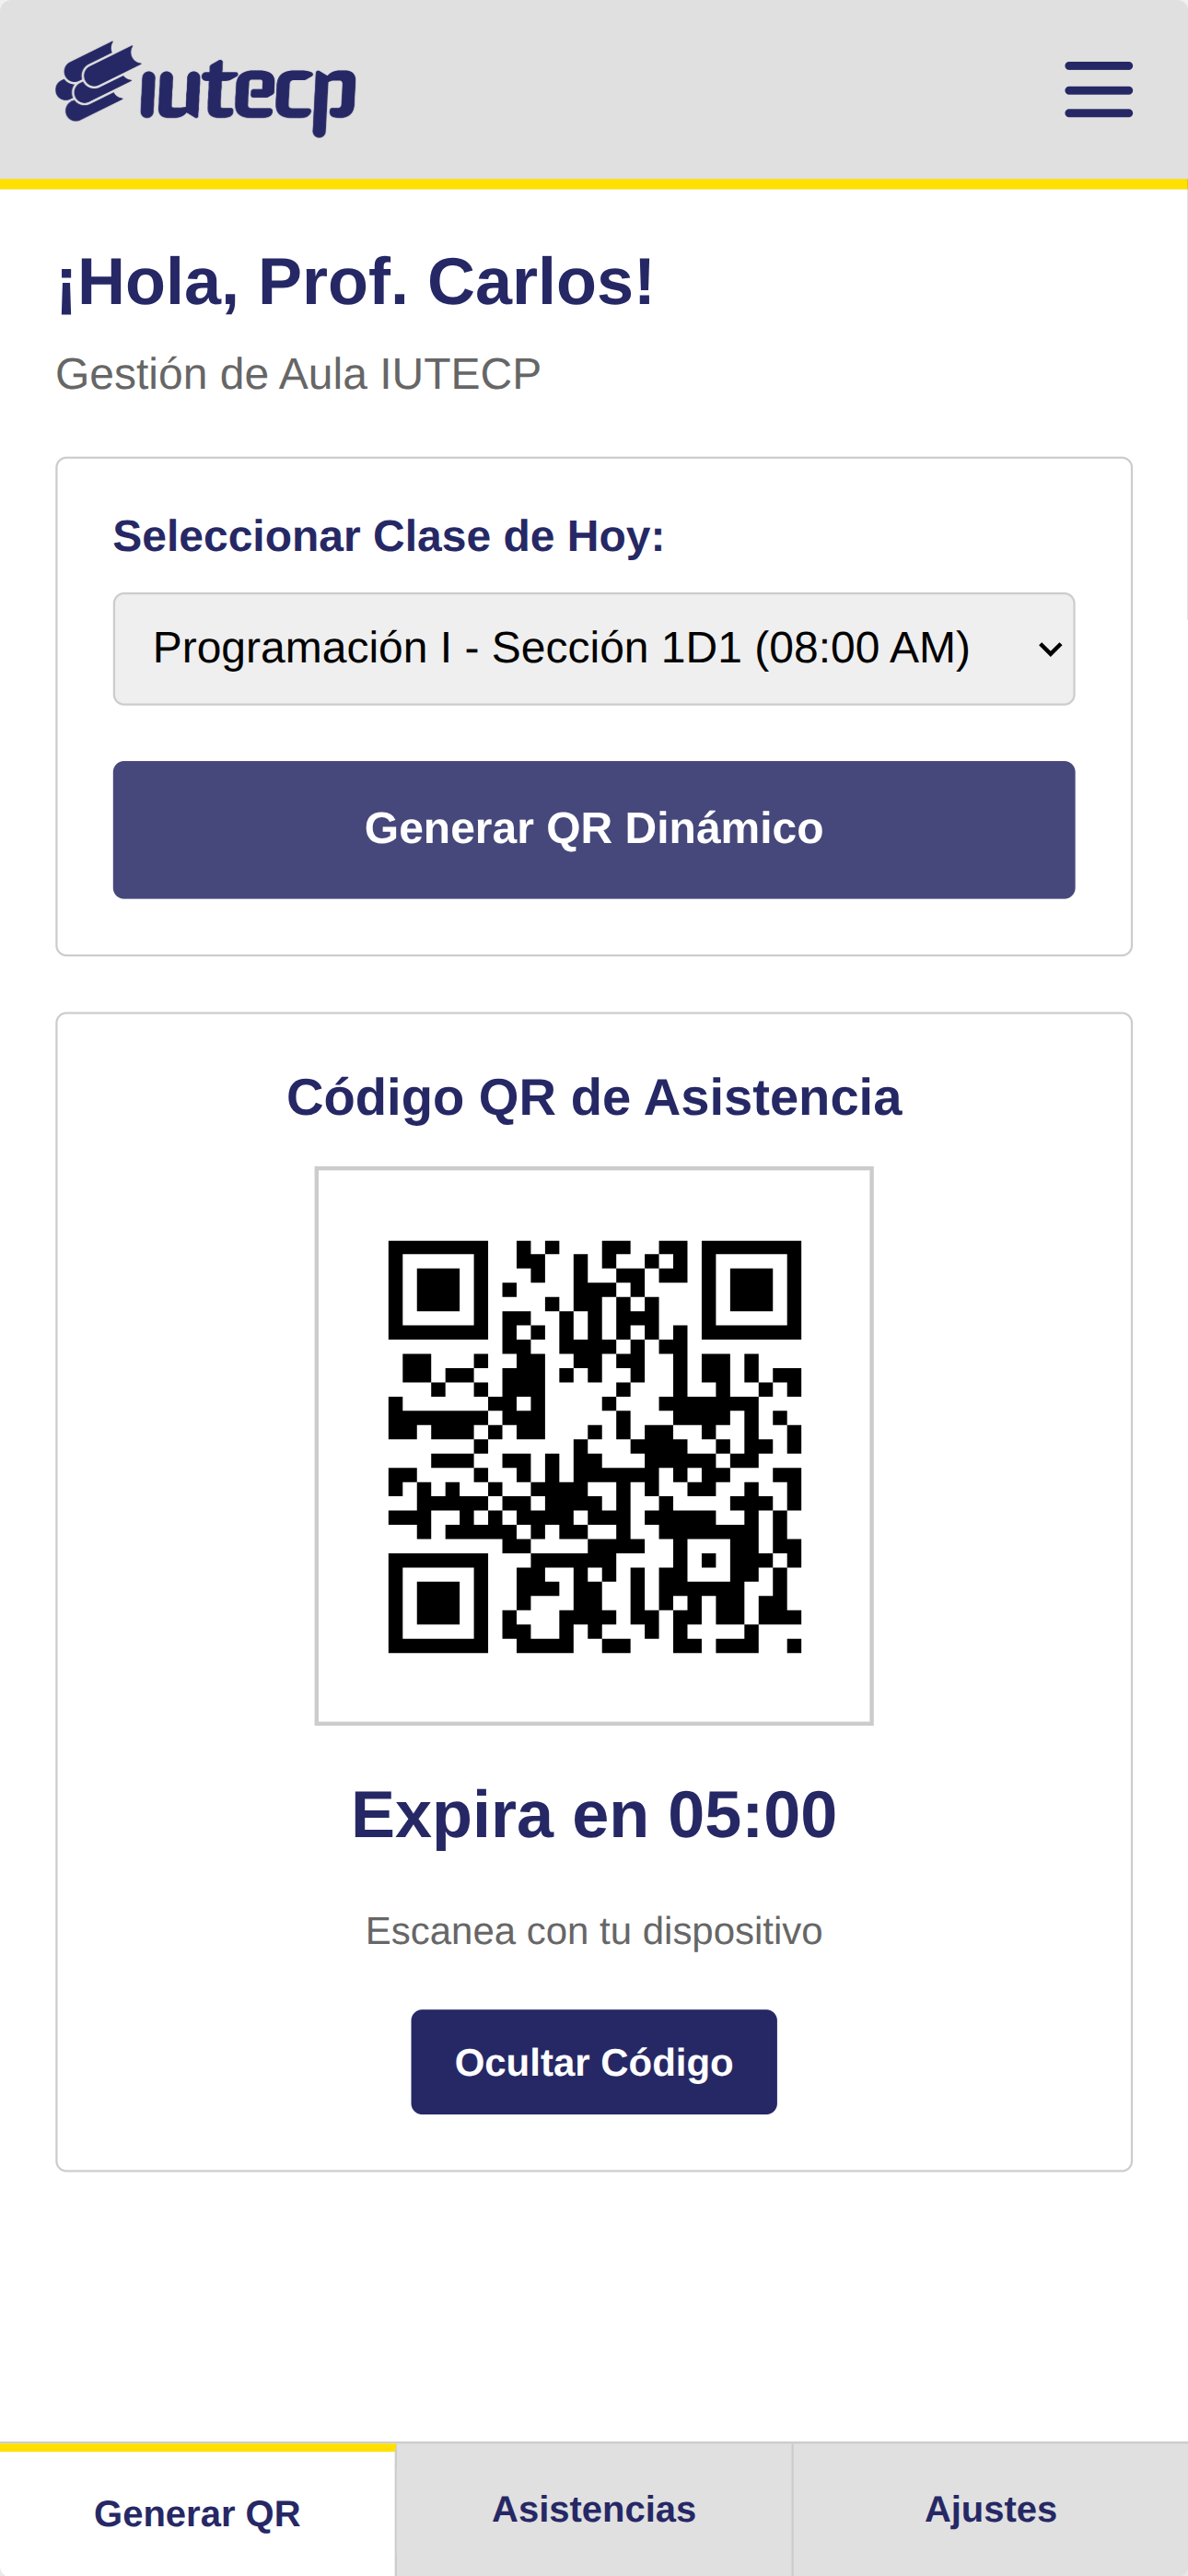
\includegraphics[width=0.3\textwidth]{../capturas/profegenerar_qr.png} &
  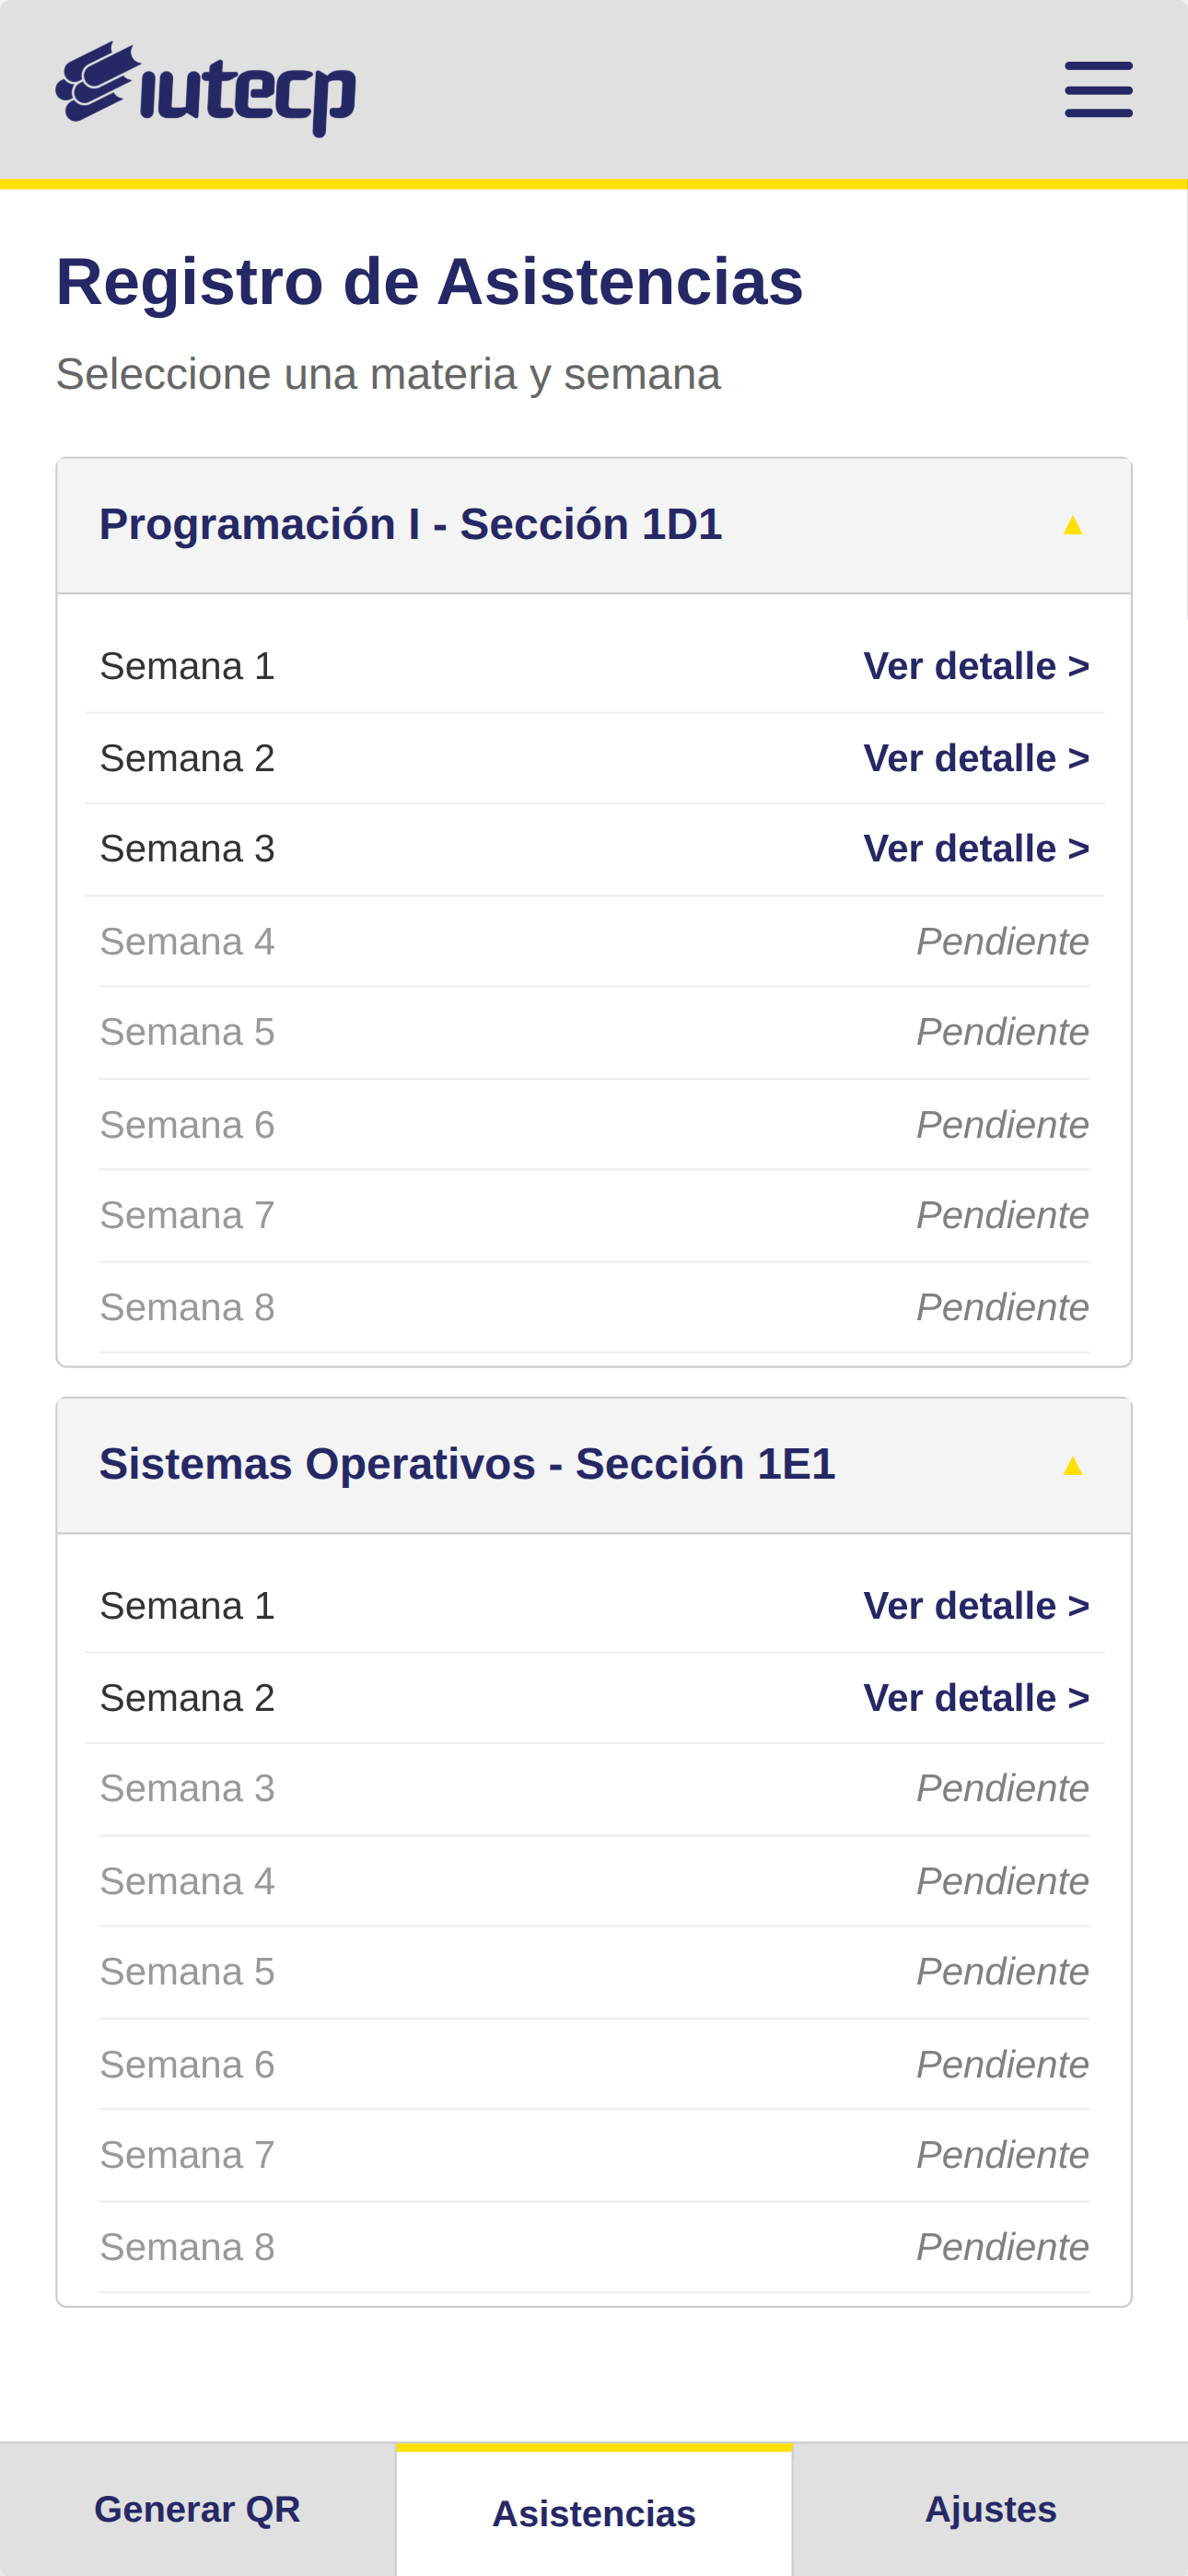
\includegraphics[width=0.3\textwidth]{../capturas/profeasistencias.png} &
  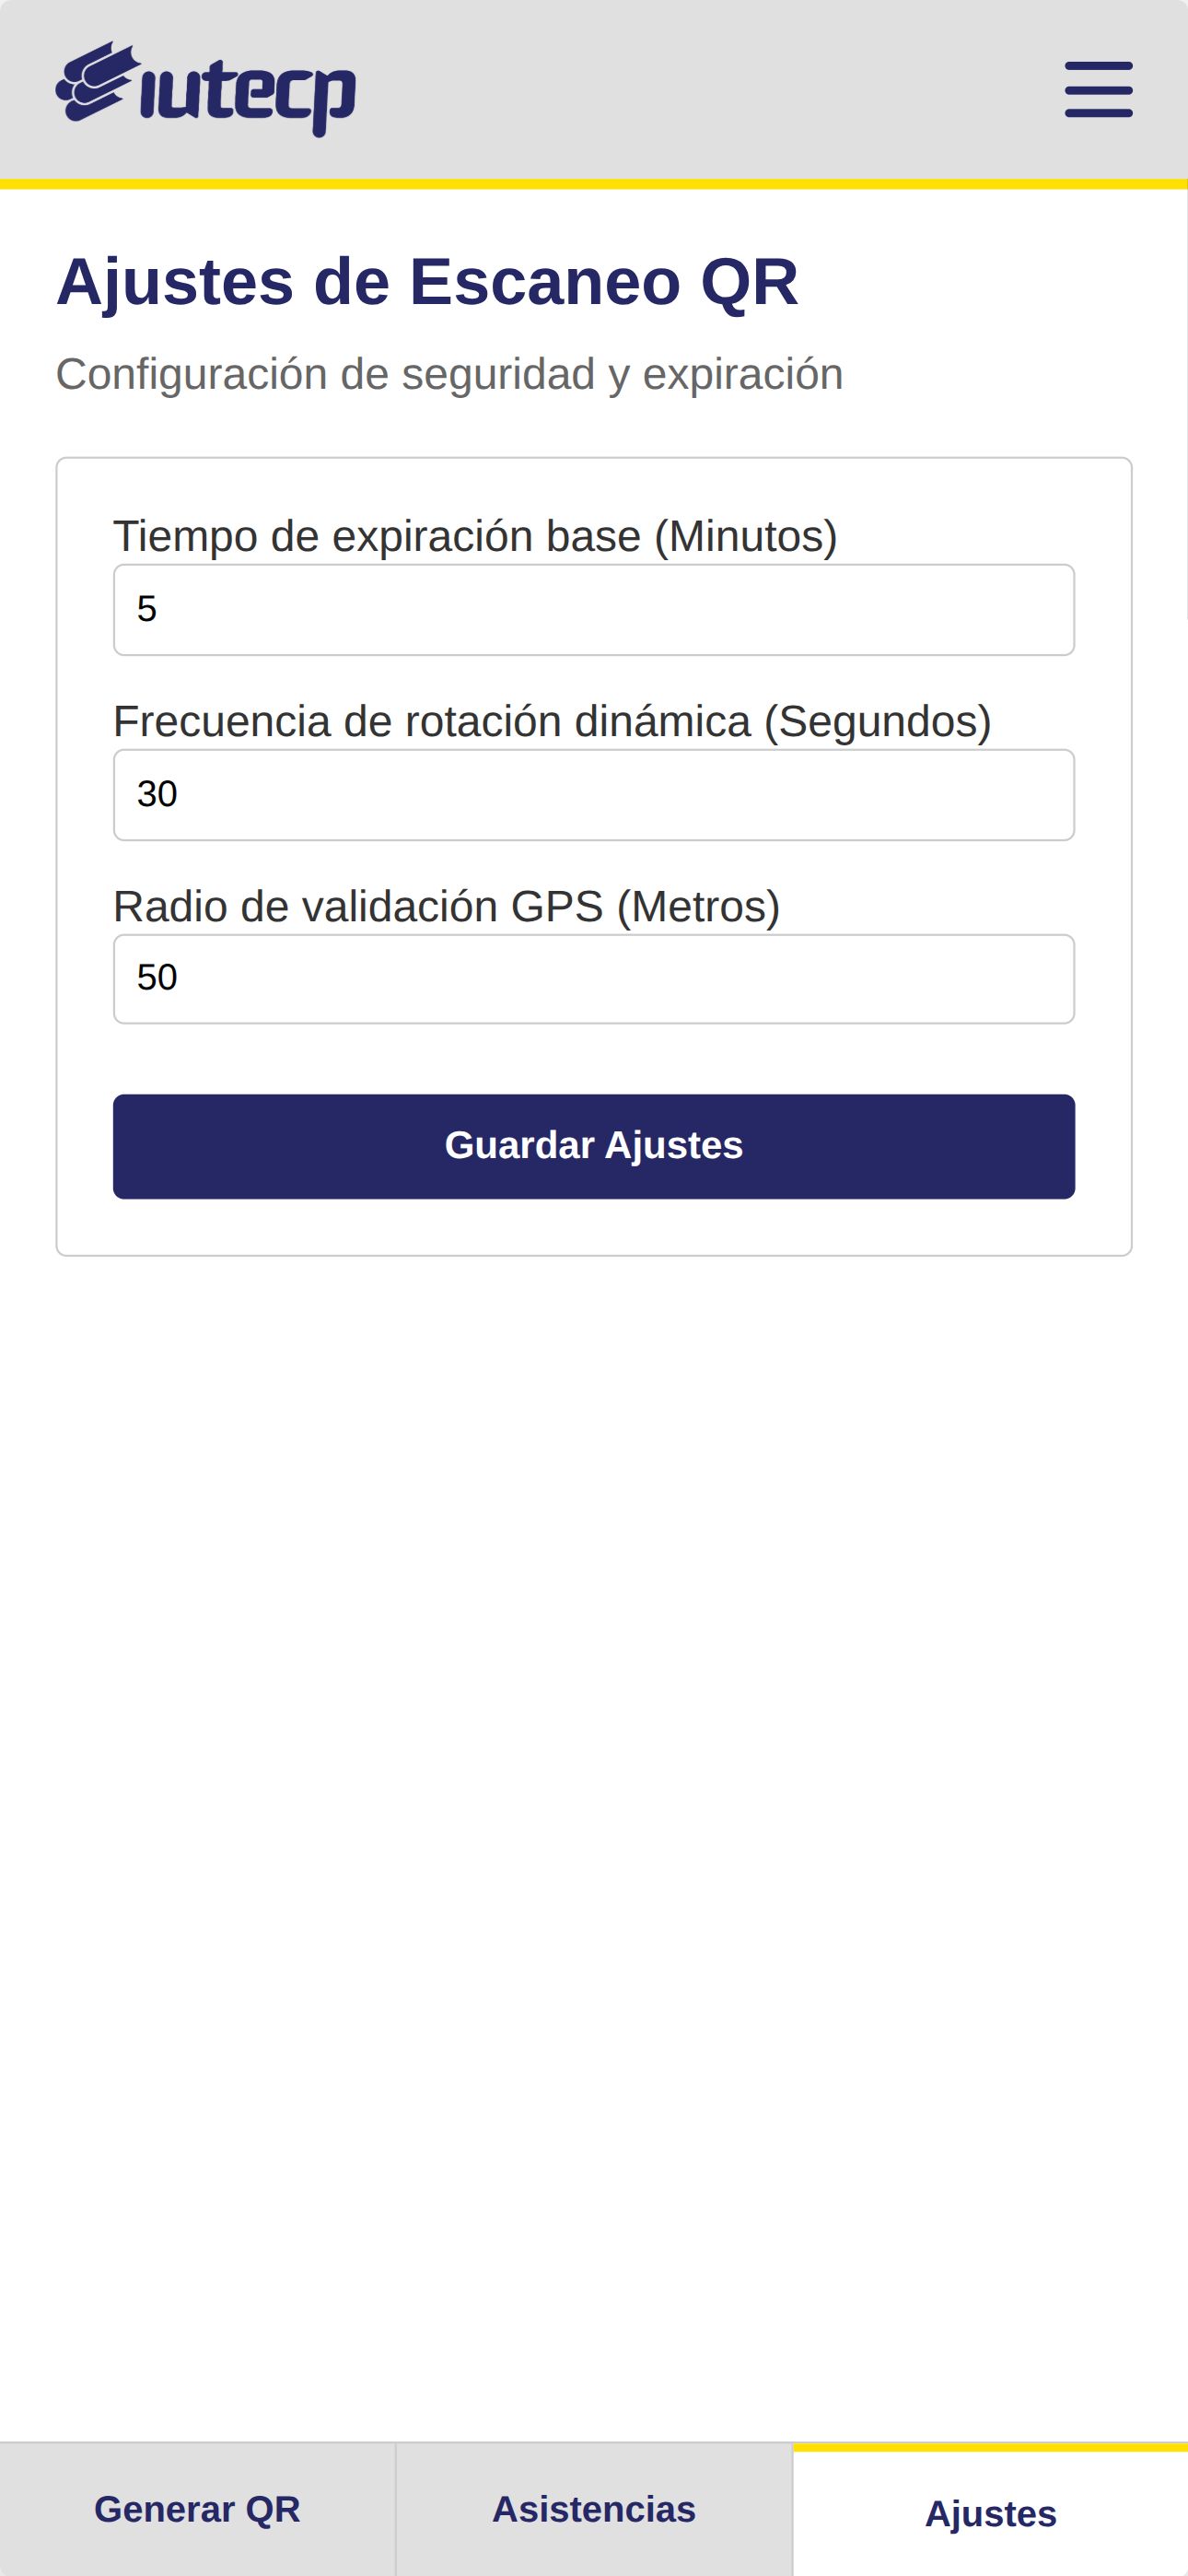
\includegraphics[width=0.3\textwidth]{../capturas/profeajustes.png} \\[2pt]
  \footnotesize\textbf{Profesor:} Generaci\'on QR &
  \footnotesize\textbf{Profesor:} Asistencias &
  \footnotesize\textbf{Profesor:} Ajustes \\[0.4cm]
  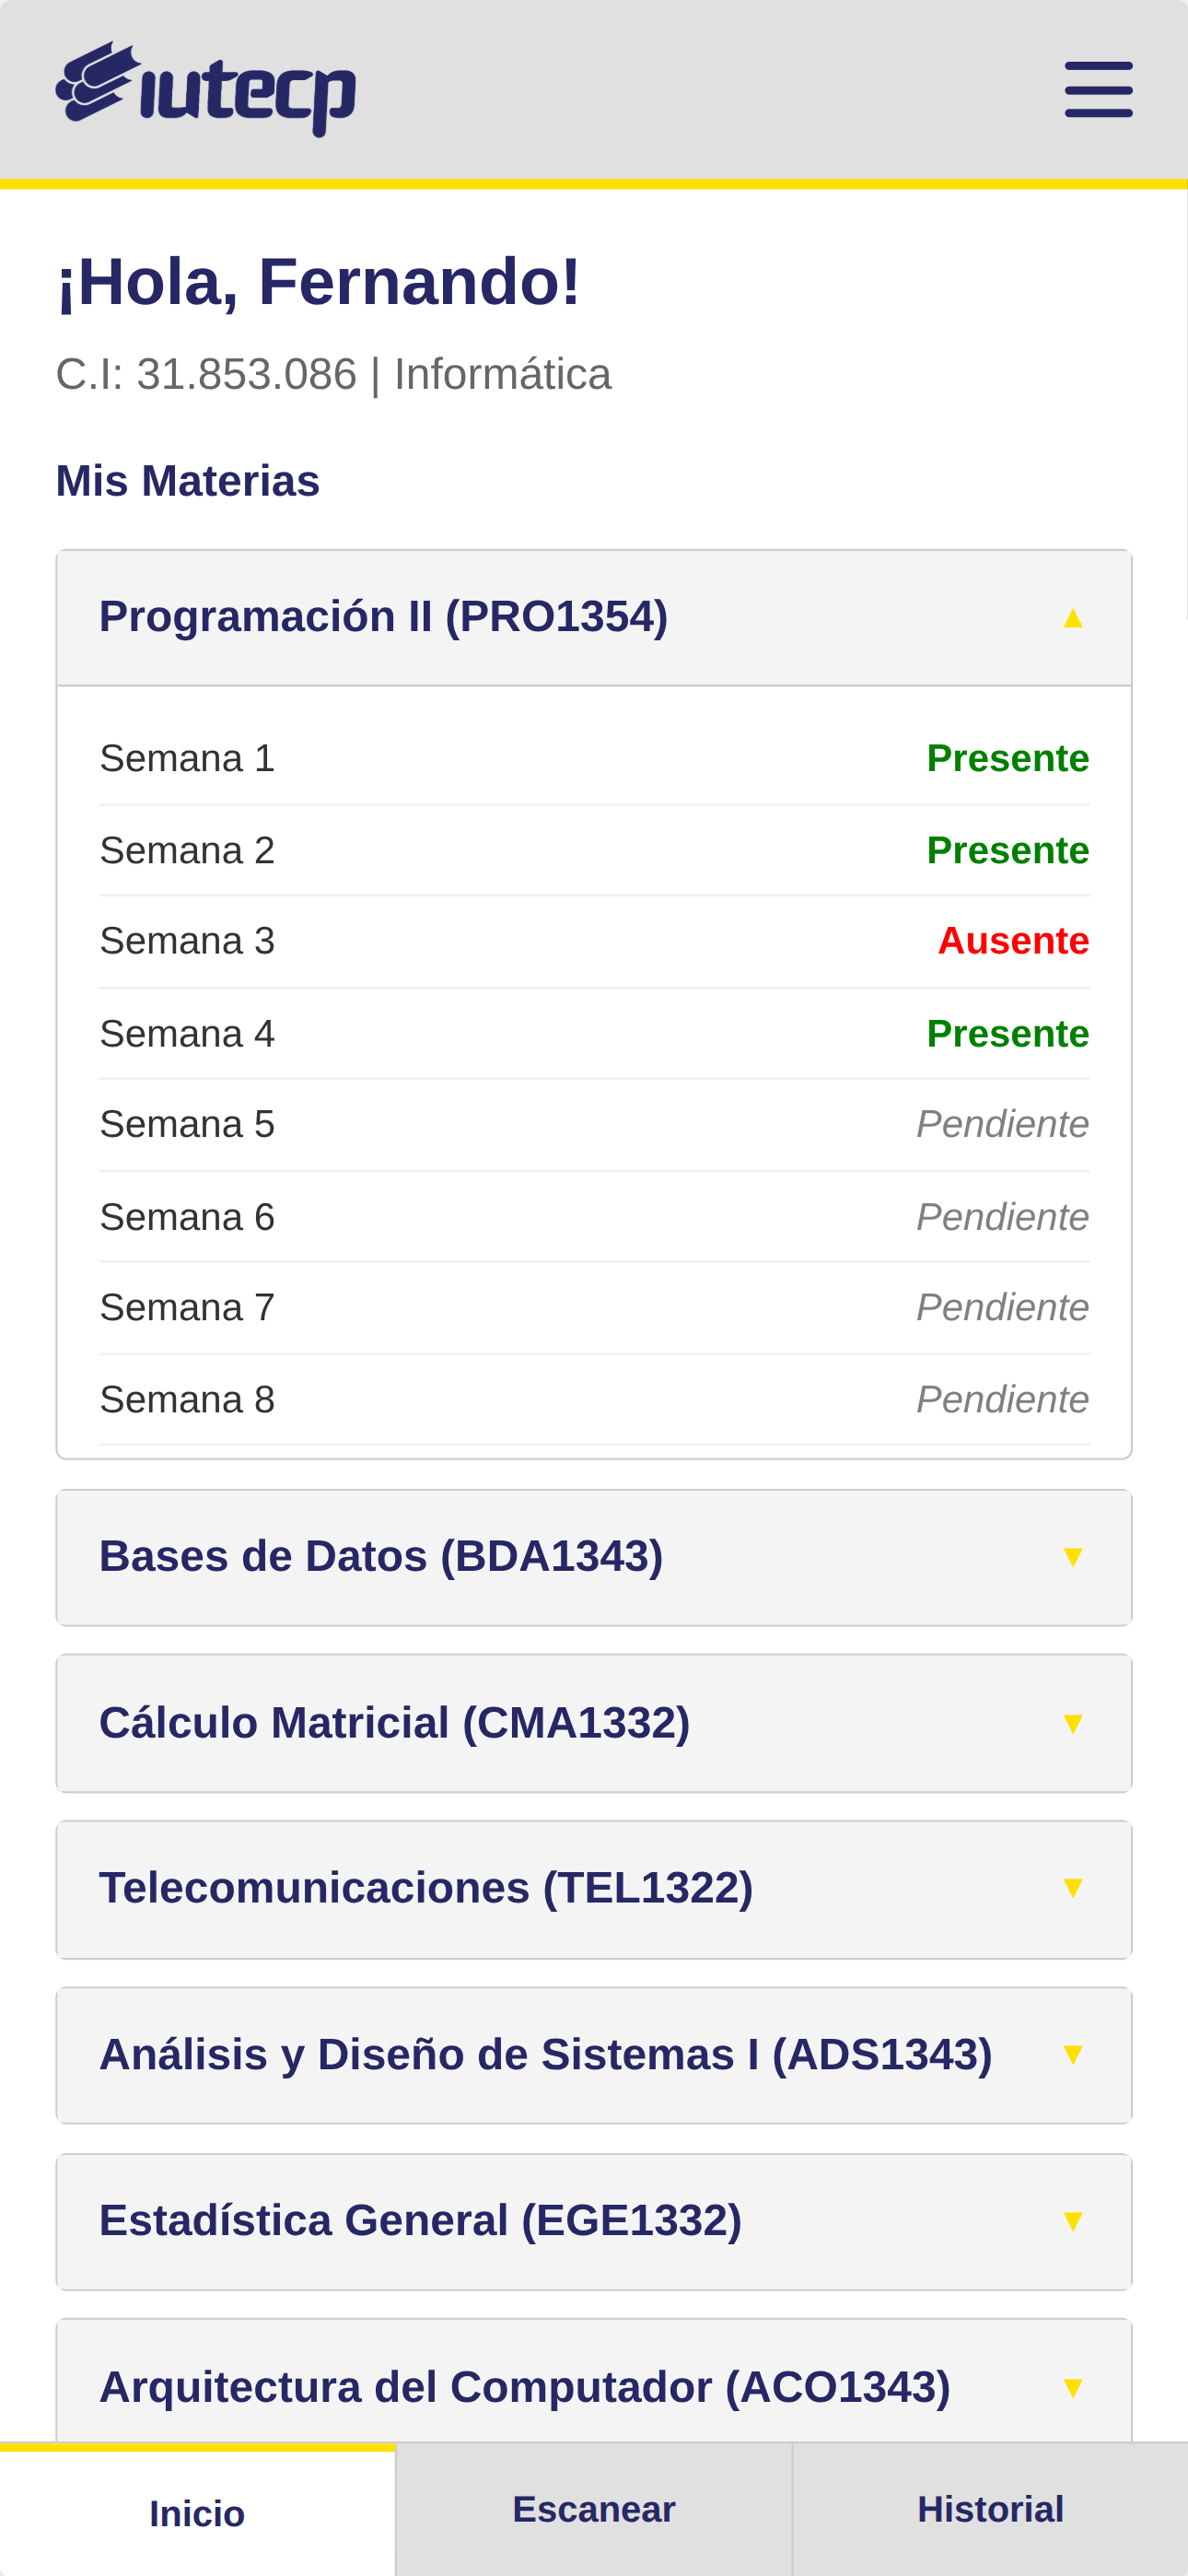
\includegraphics[width=0.3\textwidth]{../capturas/alumnoinicio.png} &
  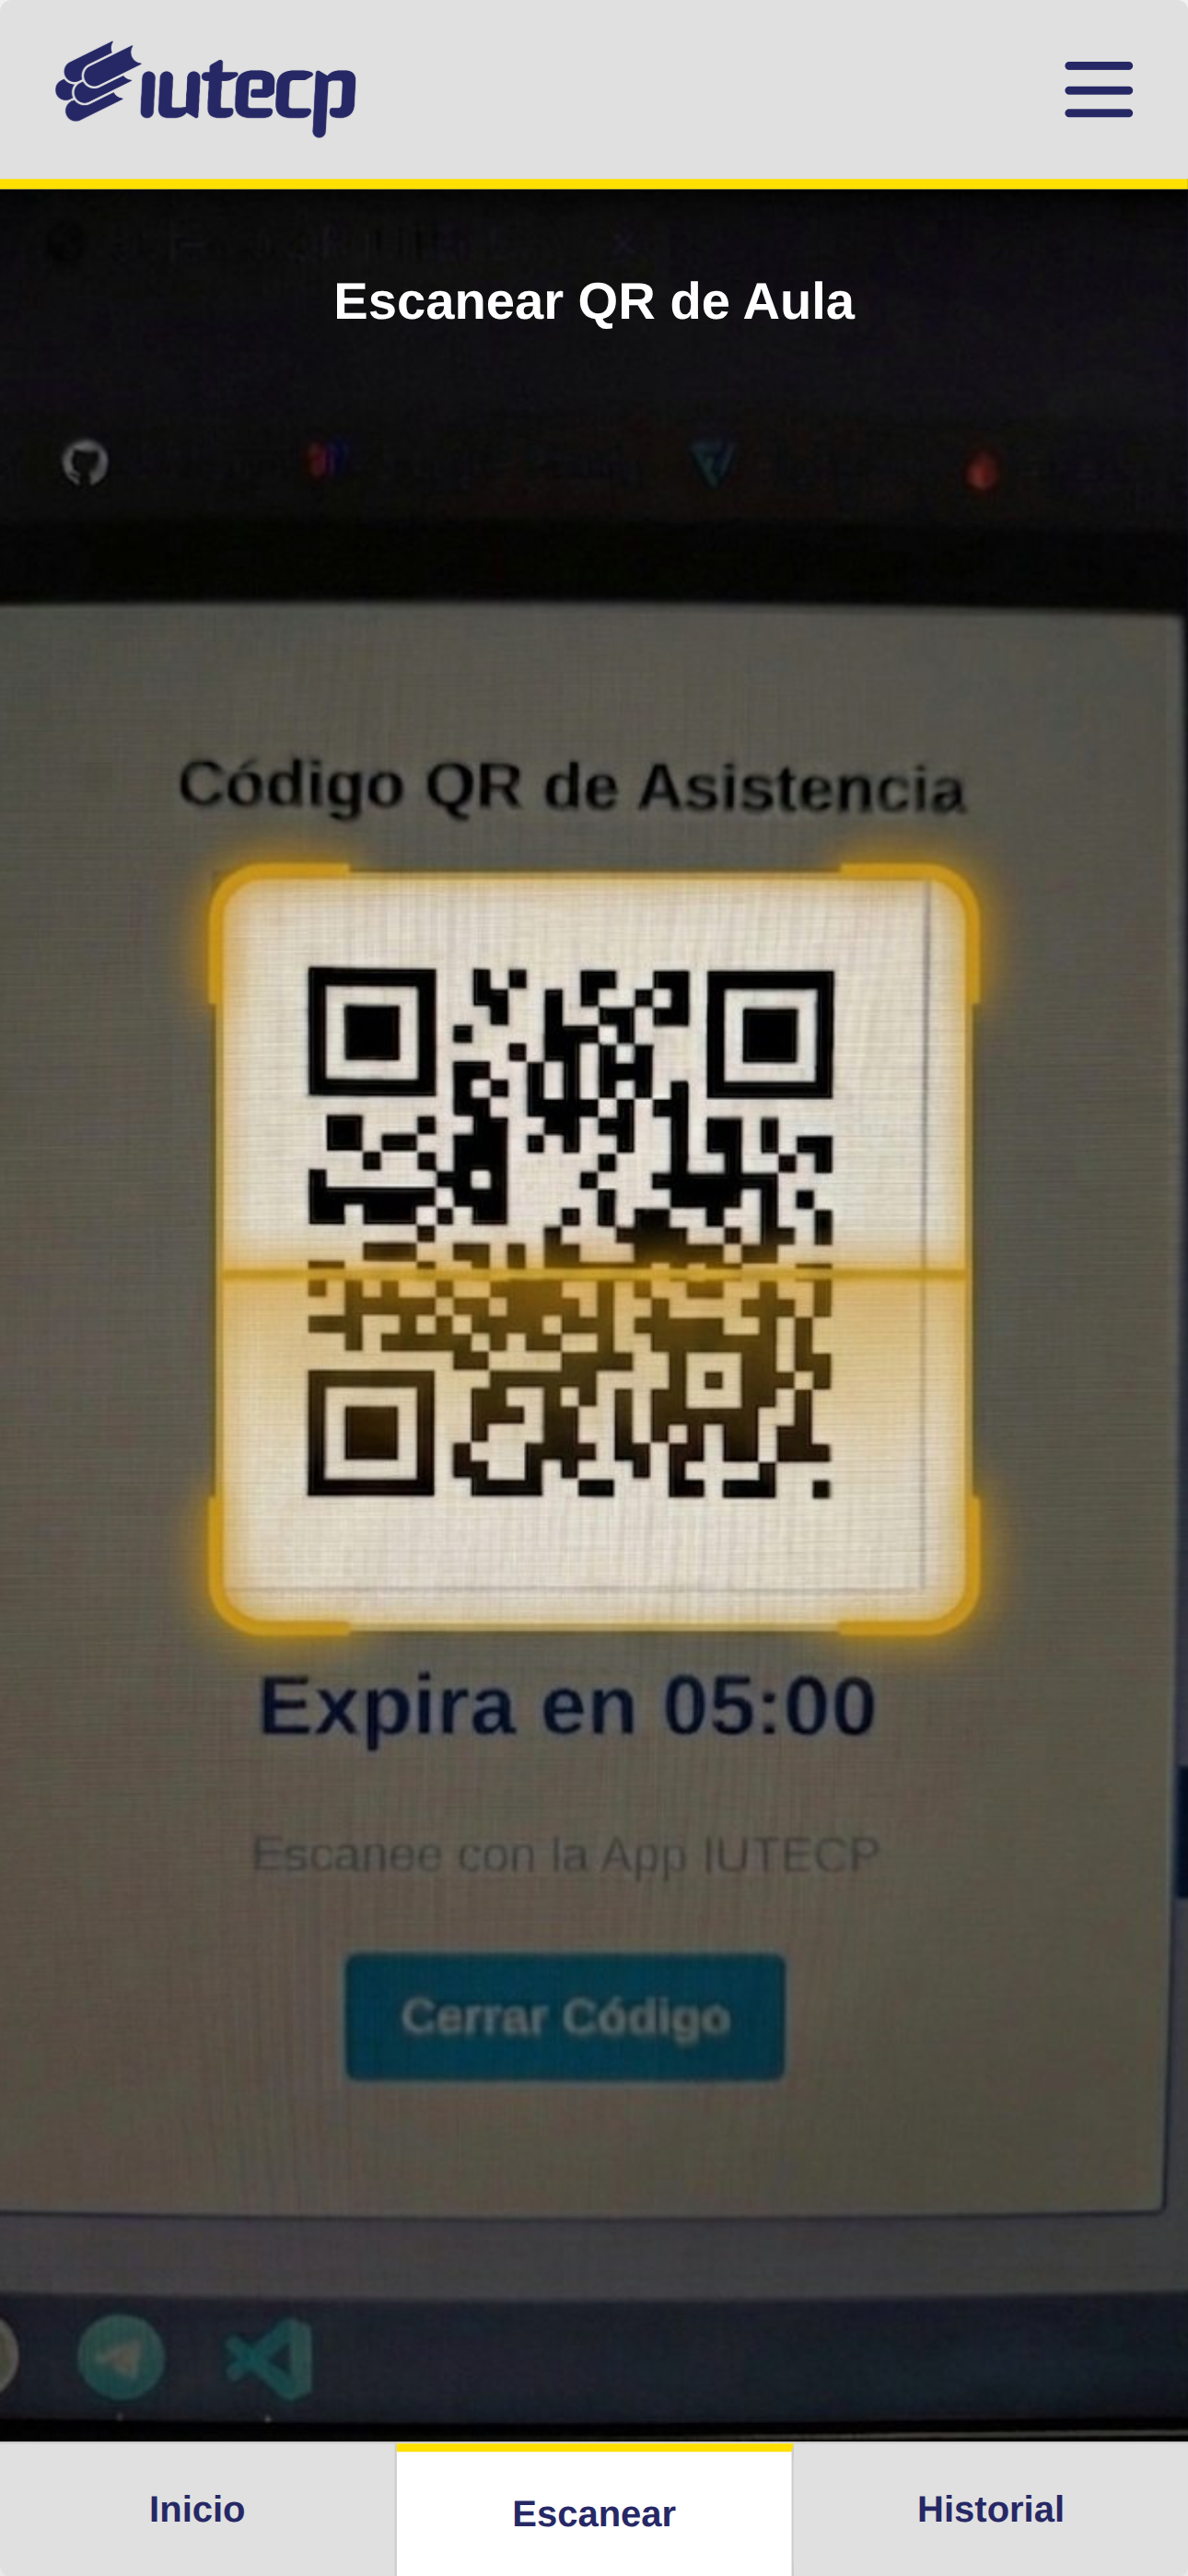
\includegraphics[width=0.3\textwidth]{../capturas/alumnoescaneo.png} &
  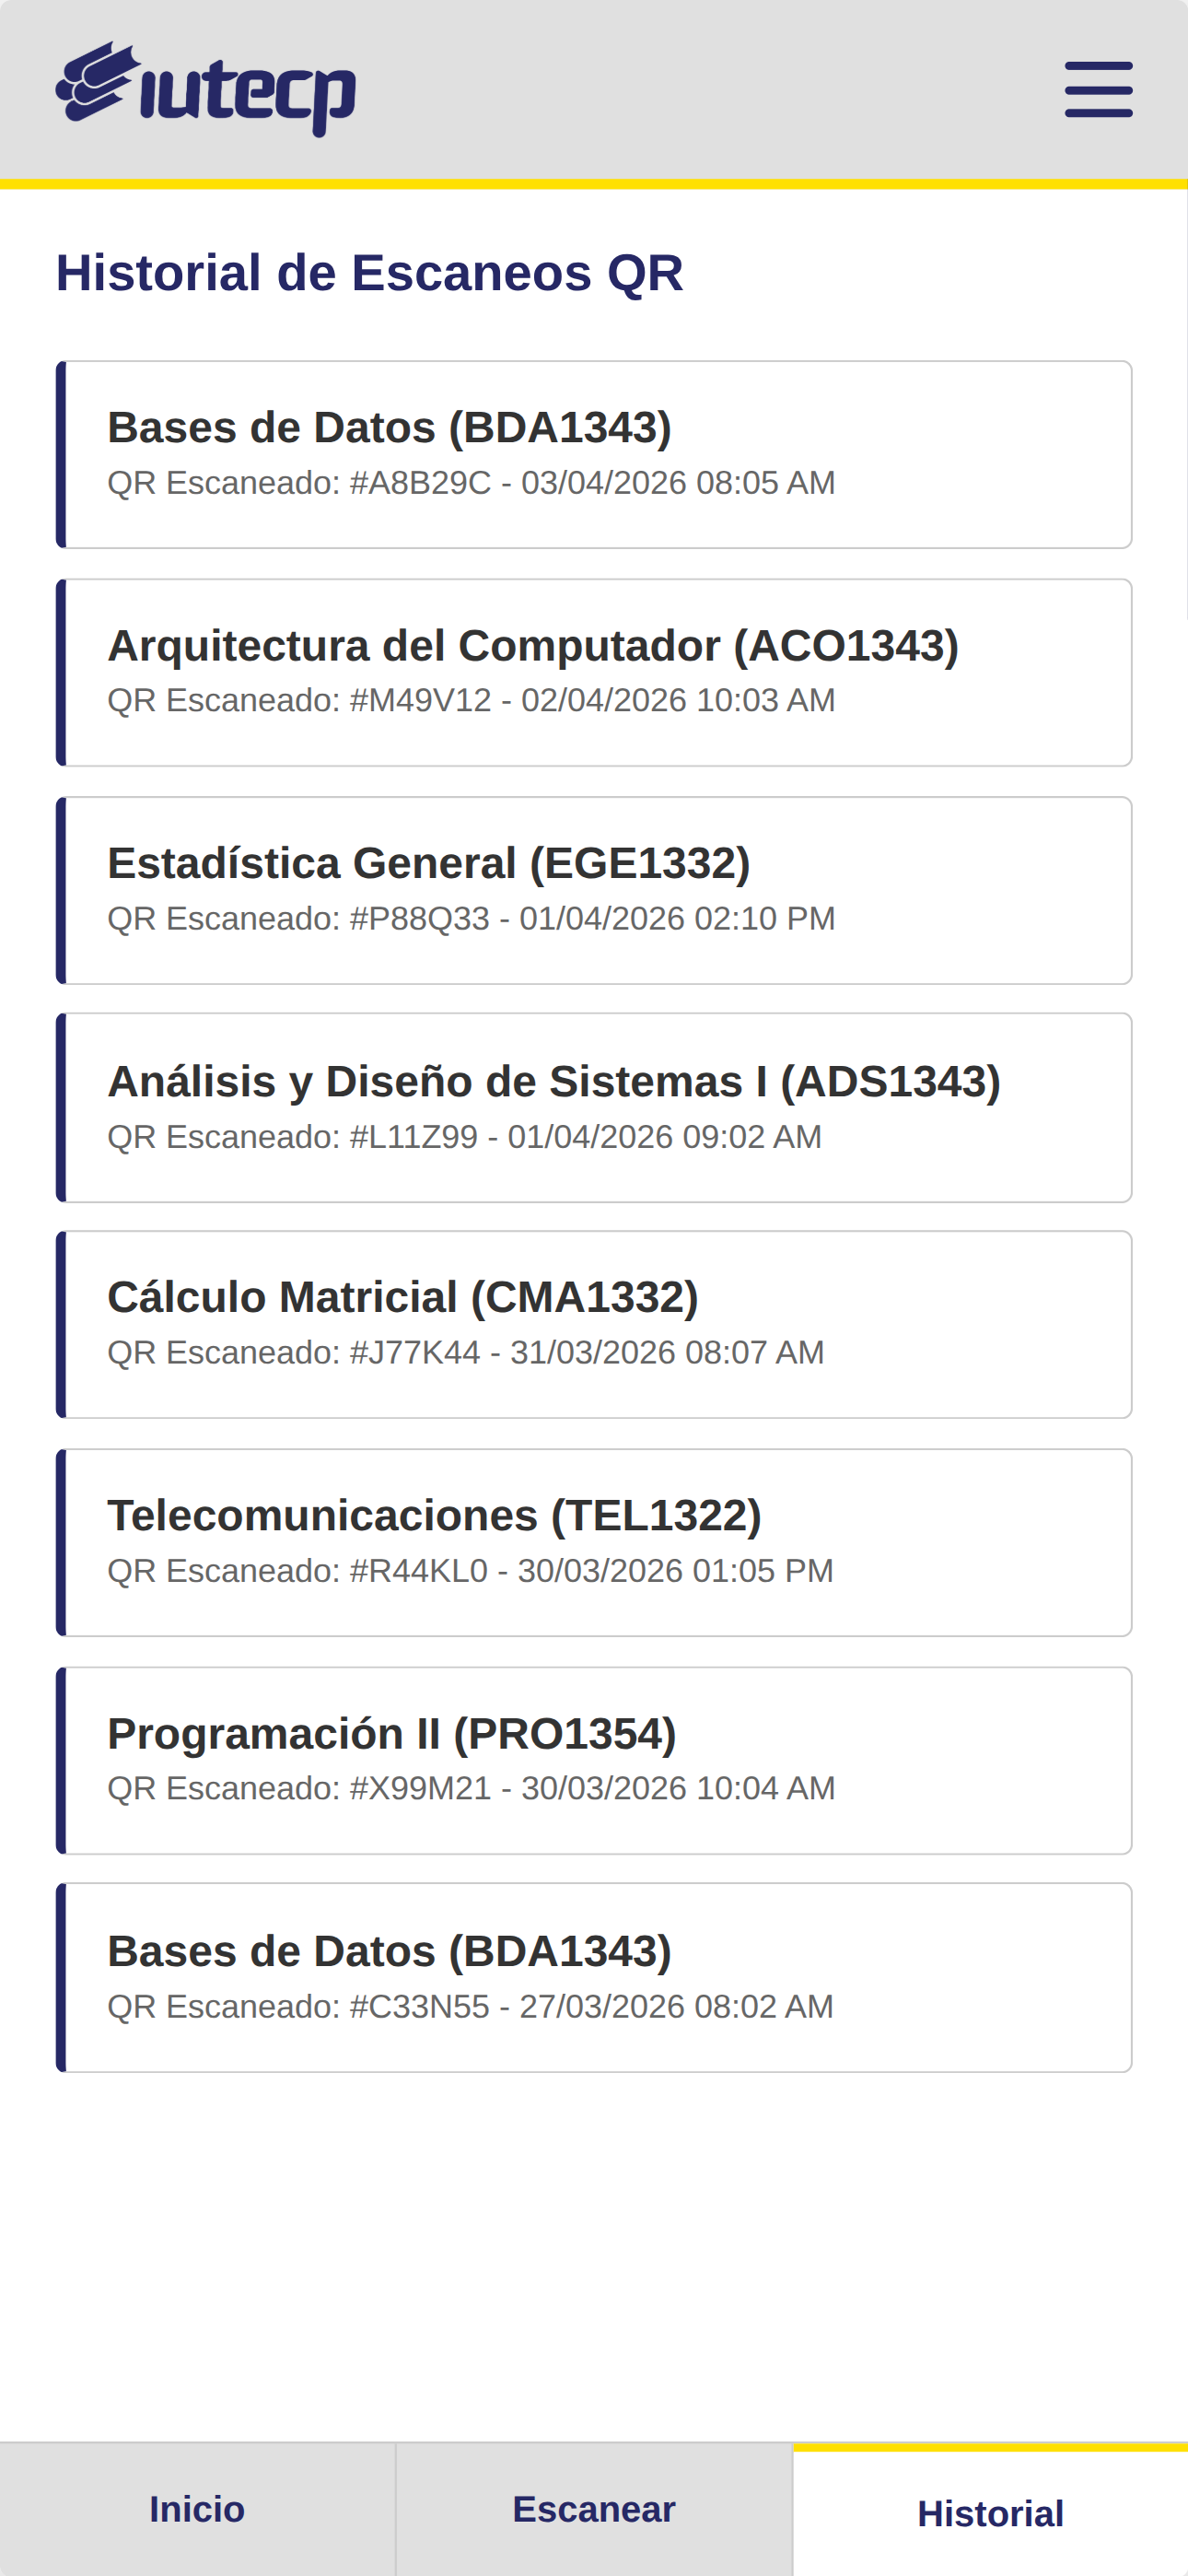
\includegraphics[width=0.3\textwidth]{../capturas/alumnohistorial.png} \\[2pt]
  \footnotesize\textbf{Estudiante:} Inicio &
  \footnotesize\textbf{Estudiante:} Escaneo QR &
  \footnotesize\textbf{Estudiante:} Historial
\end{tabular}
\end{center}

\newpage

\subsection*{Interfaces del Administrador}

\begin{center}
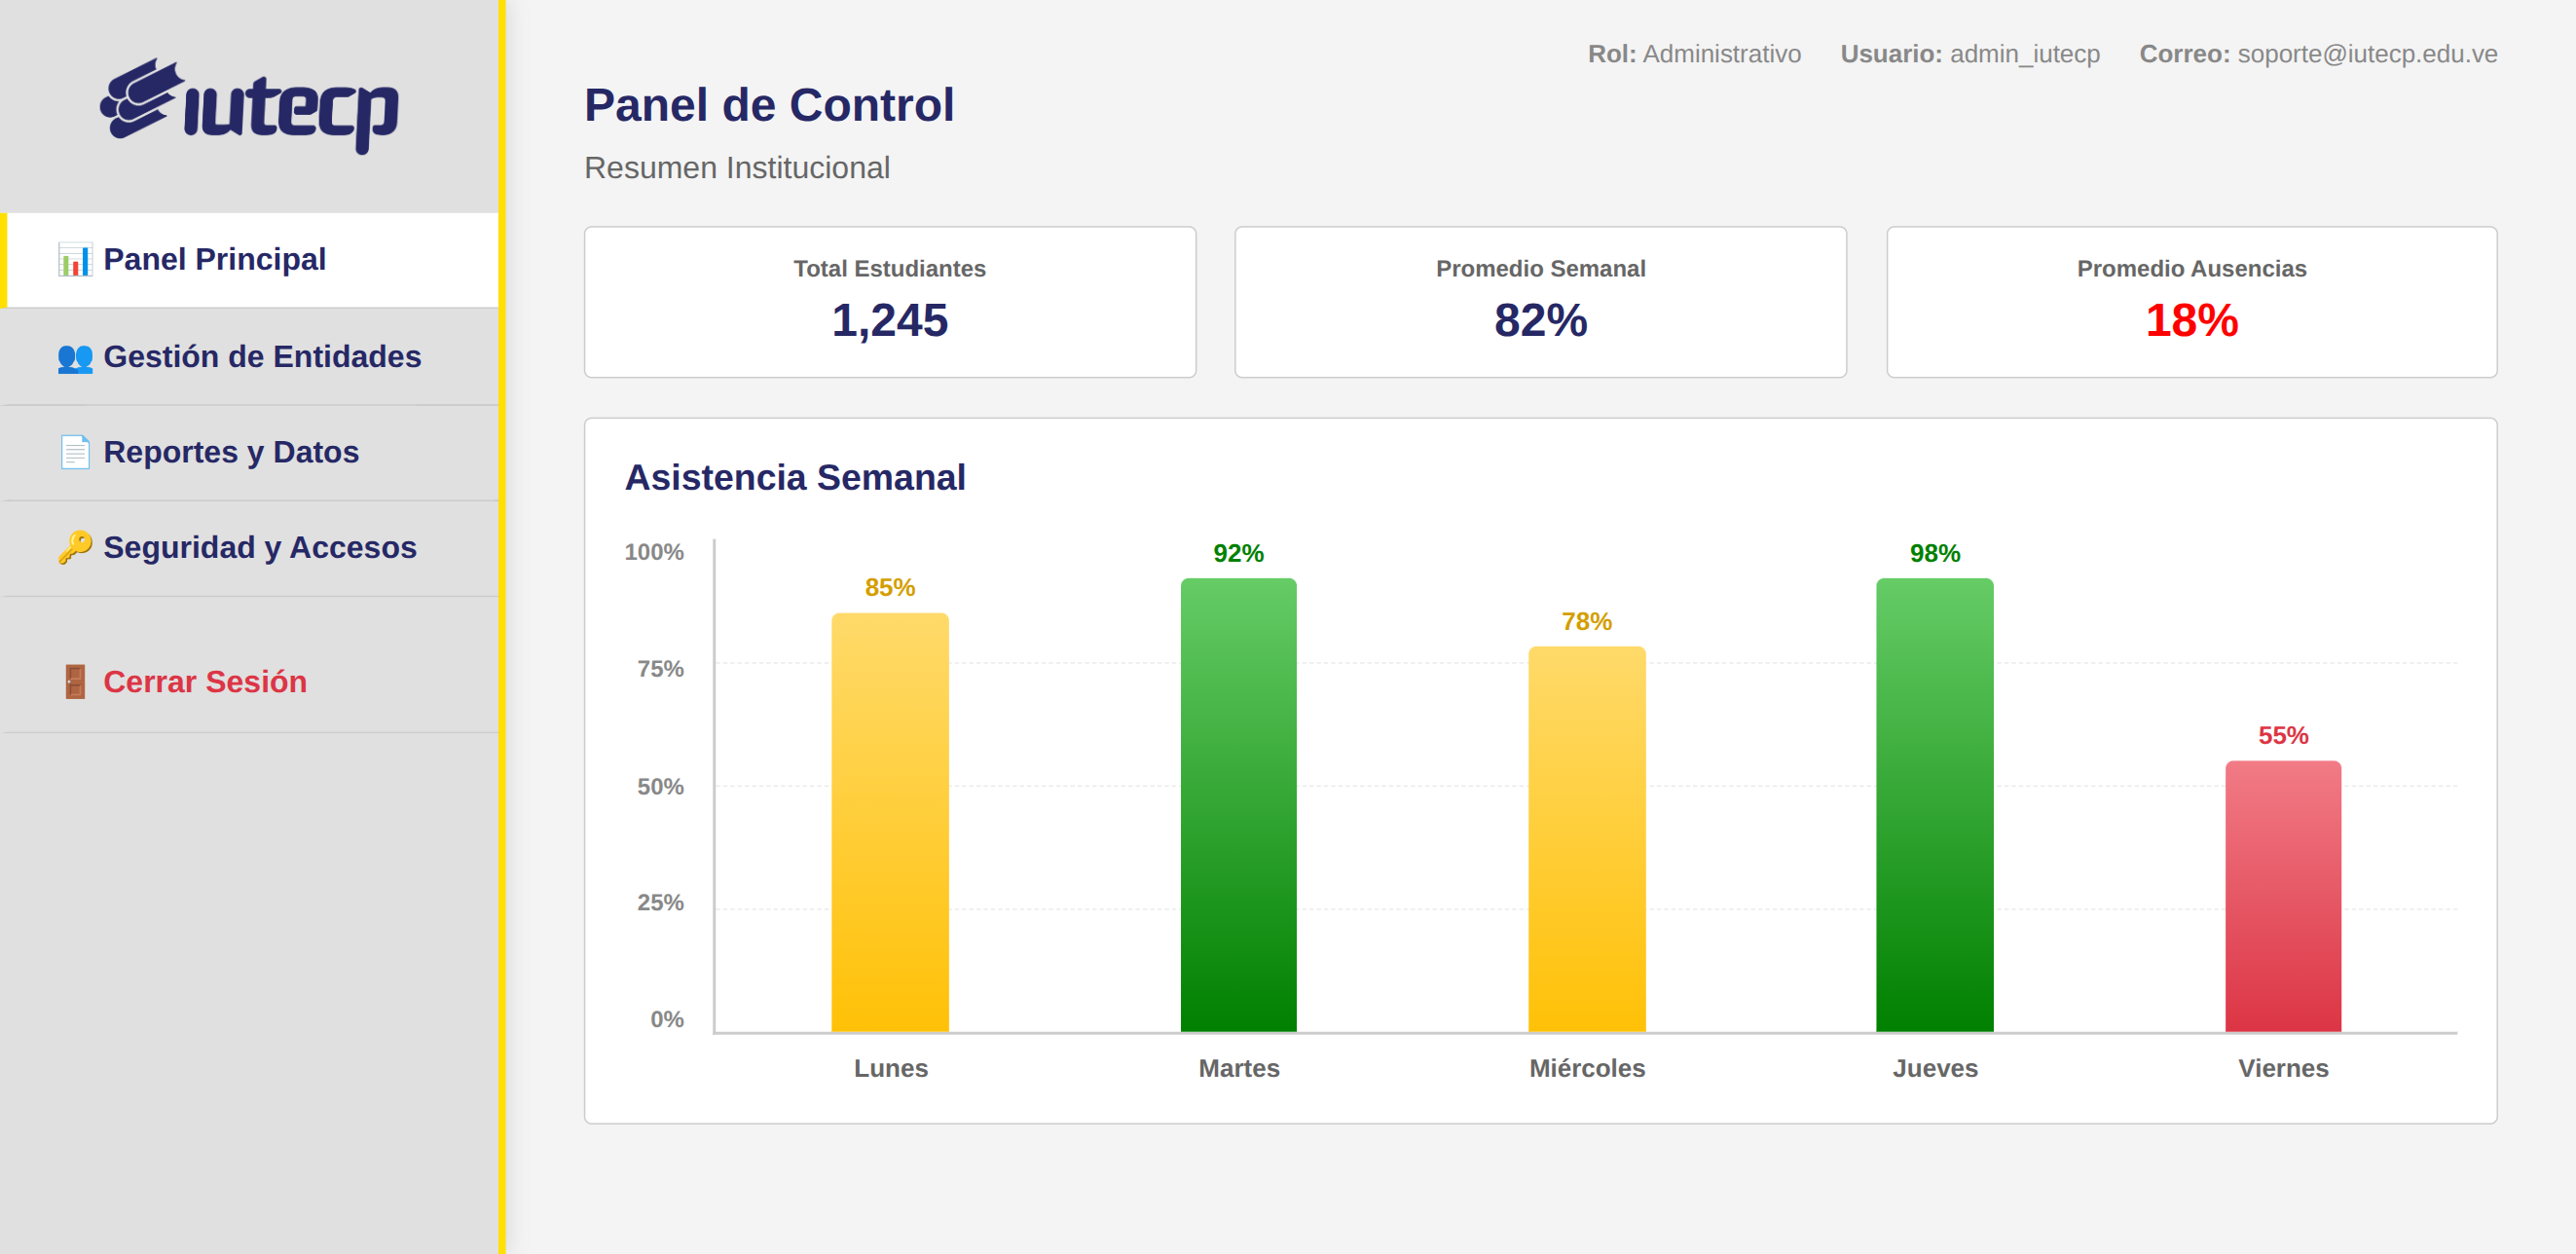
\includegraphics[width=0.8\textwidth]{../capturas/1panel_principal.png}

\vspace{0.2cm}

\textbf{Panel principal}

\vspace{0.3cm}

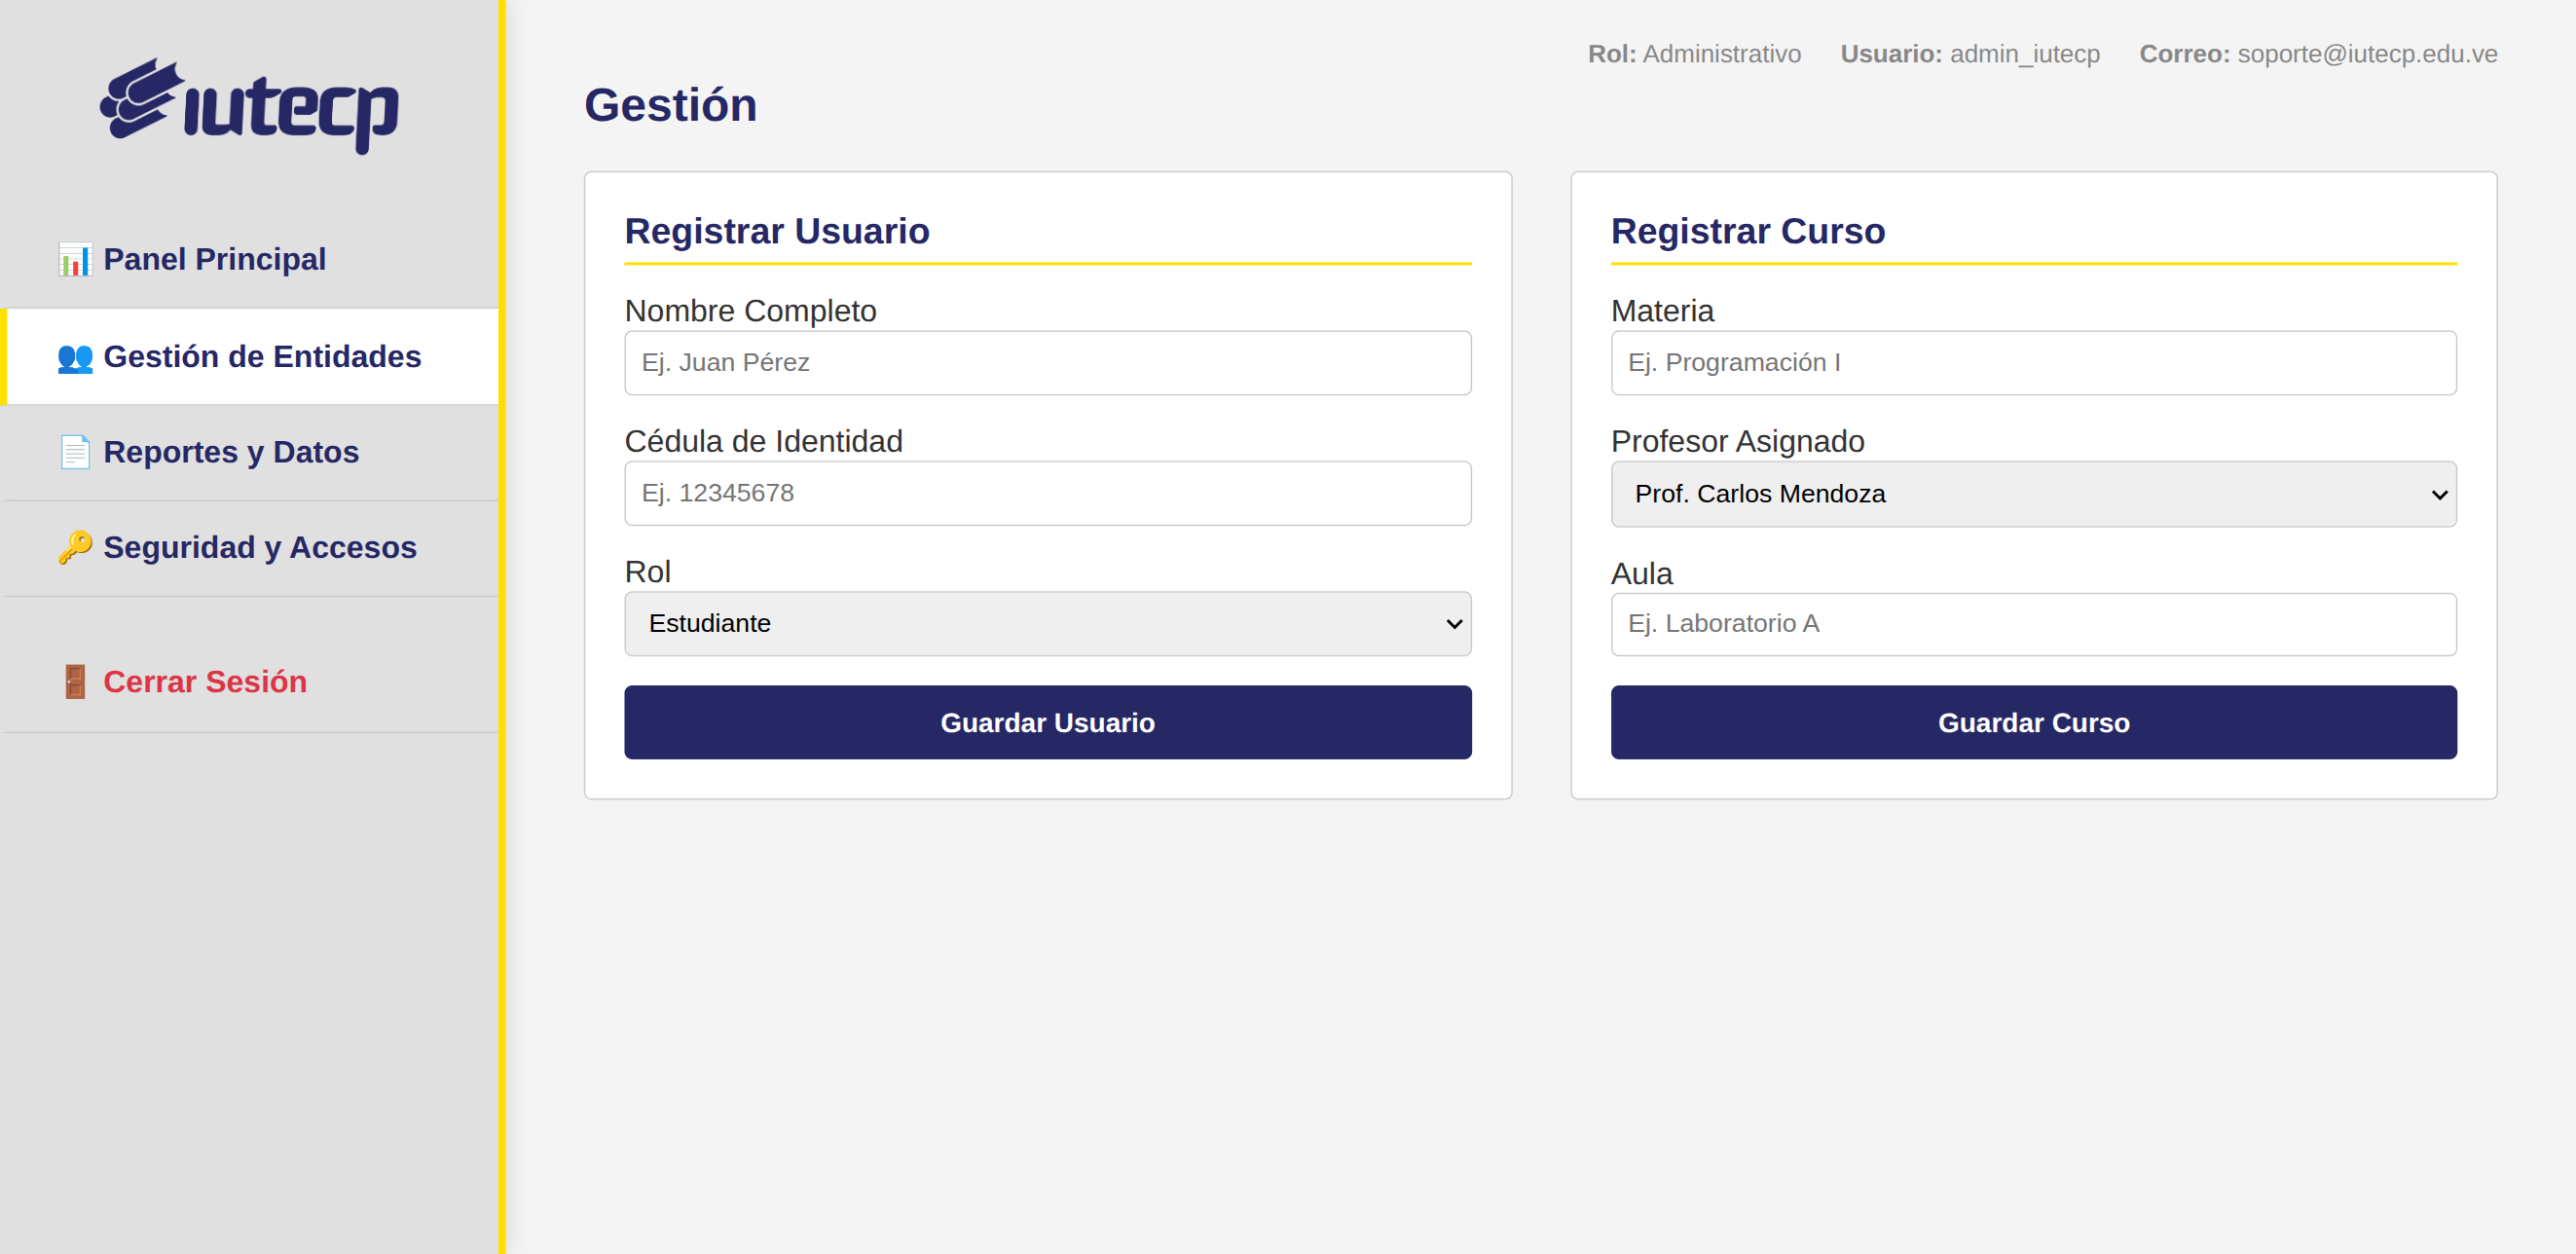
\includegraphics[width=0.8\textwidth]{../capturas/2gestion_de_entidades.png}

\vspace{0.2cm}

\textbf{Gesti\'on de entidades}

\vspace{0.3cm}

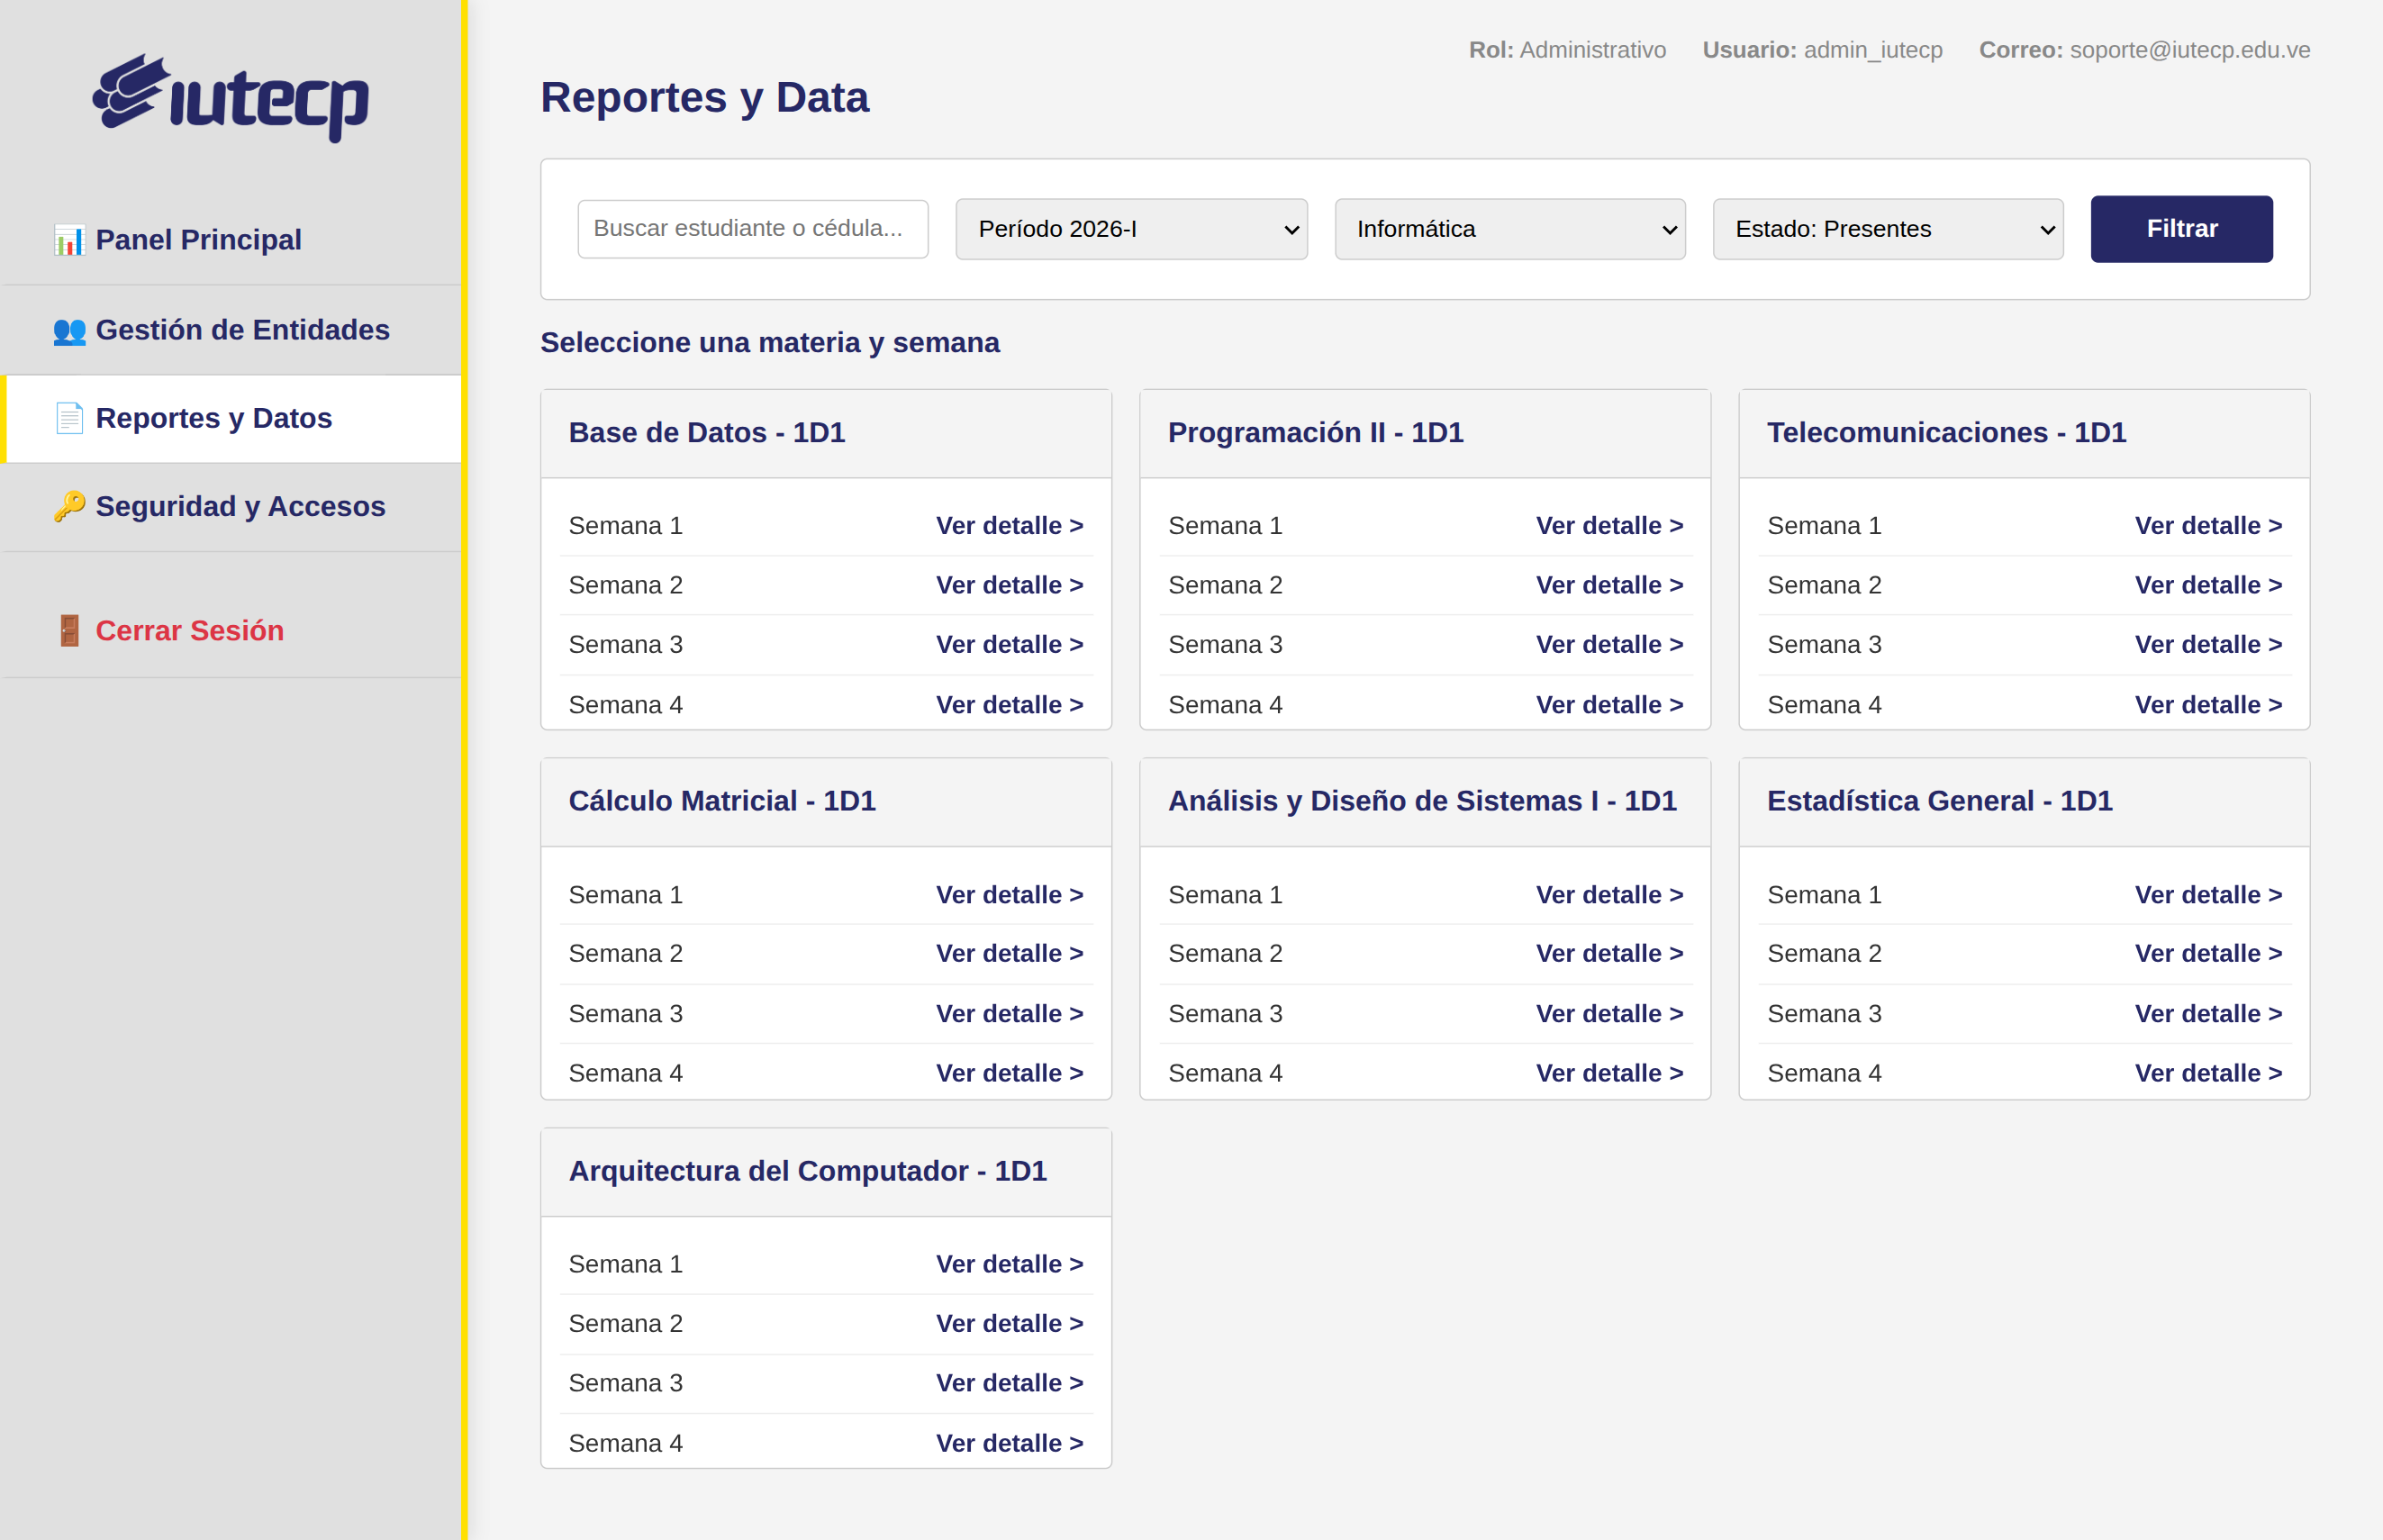
\includegraphics[width=0.8\textwidth]{../capturas/3reportes_y_datos.png}

\vspace{0.2cm}

\textbf{Reportes y datos}

\vspace{0.3cm}

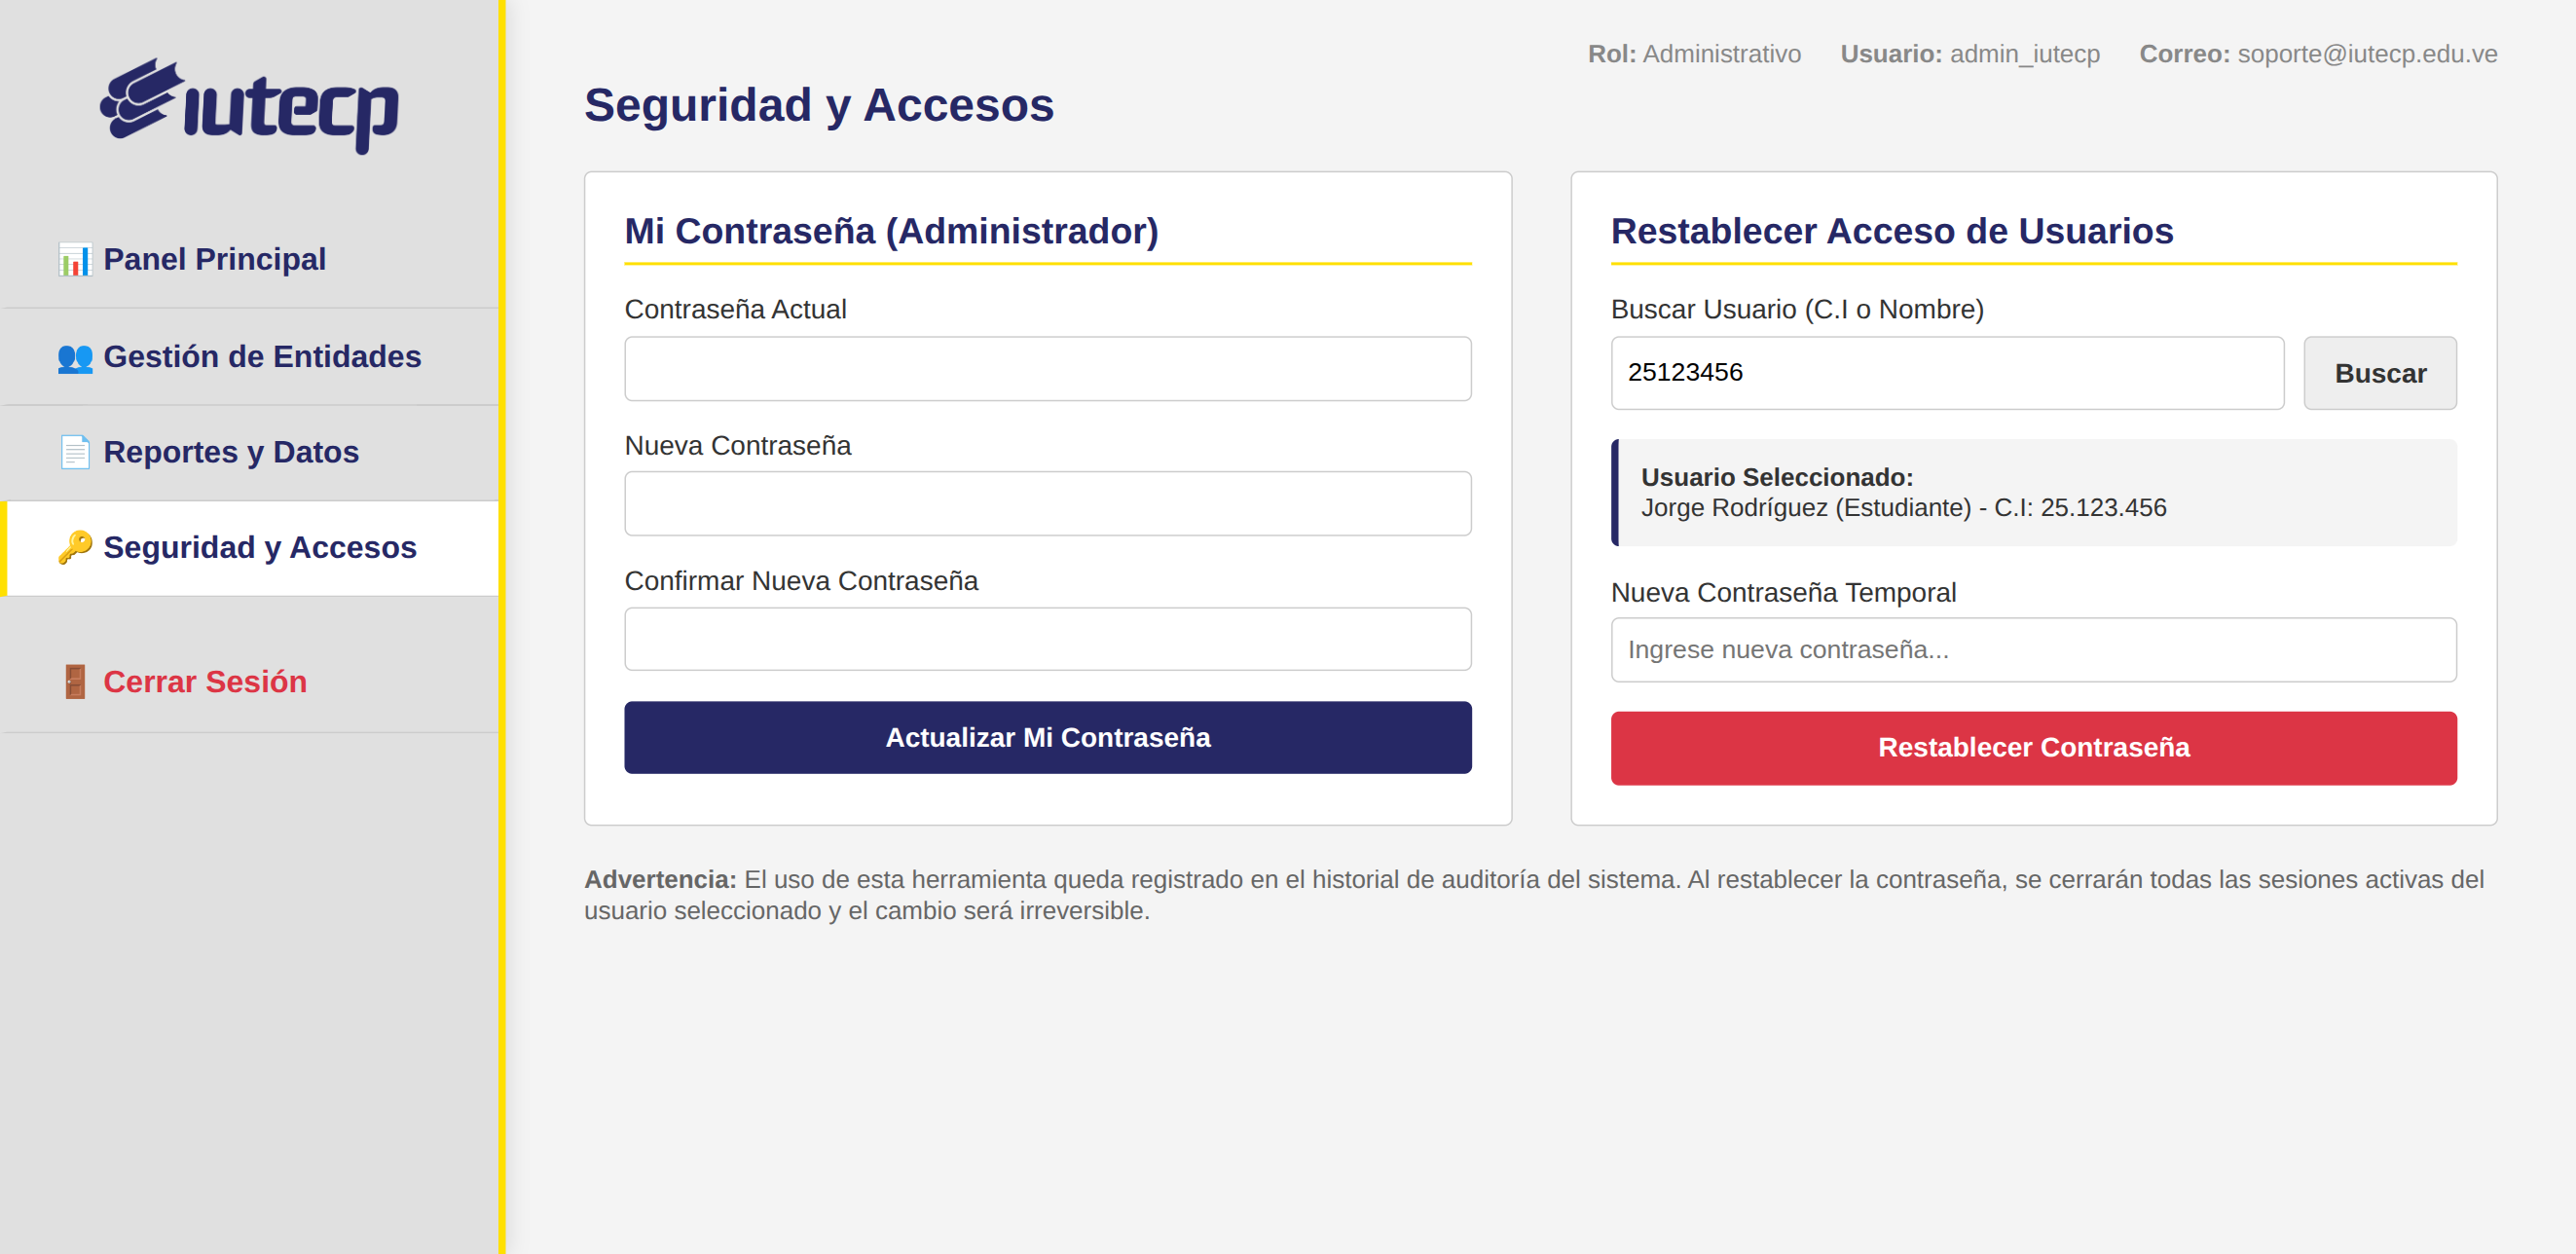
\includegraphics[width=0.8\textwidth]{../capturas/4seguridad_y_accesos.png}

\vspace{0.2cm}

\textbf{Seguridad y accesos}
\end{center}

\newpage

% ============================================================
% CAPÍTULO XIII
% ============================================================
\chapter{DISE\~NO NO FUNCIONAL}

El dise\~no no funcional del sistema aborda las restricciones de calidad que garantizan un funcionamiento seguro, usable y accesible.

\section{Seguridad y Privacidad}

\subsection{Autenticaci\'on y Control de Acceso}

\begin{itemize}
  \item Las contrase\~nas se almacenan utilizando la funci\'on \texttt{password\_hash} de PHP con el algoritmo \texttt{PASSWORD\_DEFAULT}.
  \item En el primer inicio de sesi\'on, se asigna una contrase\~na temporal que debe ser cambiada obligatoriamente.
  \item Cada usuario posee un rol (administrador, profesor o estudiante) que determina los m\'odulos y acciones a los que tiene acceso.
  \item Las cuentas pueden ser desactivadas por el administrador, impidiendo el acceso incluso con credenciales v\'alidas.
  \item El administrador no puede autodestruirse ni auto-desactivarse, garantizando la integridad del control del sistema.
\end{itemize}

\subsection{Protecci\'on contra Ataques}

\begin{itemize}
  \item Las consultas a la base de datos utilizan sentencias preparadas (PDO), eliminando el riesgo de inyecci\'on SQL.
  \item Los datos ingresados por los usuarios se sanitizan para neutralizar intentos de inyecci\'on de c\'odigo malicioso (XSS).
  \item Los c\'odigos QR se generan con entrop\'ia criptogr\'afica y expiraci\'on configurable, asoci\'andose a una sesi\'on de clase \'unica para impedir su reutilizaci\'on.
\end{itemize}

\subsection{Auditor\'ia}

El sistema registra todas las acciones relevantes en una tabla de auditor\'ia que almacena: identificador del usuario, tipo de acci\'on, descripci\'on detallada, direcci\'on IP y marca de tiempo. Esto permite rastrear actividades inusuales y mantener un historial de uso.

\section{Usabilidad}

\begin{itemize}
  \item Las interfaces presentan una navegaci\'on jer\'arquica adaptada al rol del usuario, con paneles resumidos que permiten acceso r\'apido a las funcionalidades principales.
  \item El proceso de escaneo QR se realiza directamente desde la c\'amara del dispositivo sin instalar aplicaciones de terceros, con retroalimentaci\'on visual inmediata.
  \item Los formularios incluyen validaci\'on en tiempo real con mensajes de error espec\'ificos, y las acciones destructivas requieren confirmaci\'on previa.
\end{itemize}

\section{Accesibilidad}

\begin{itemize}
  \item Las interfaces se adaptan a diferentes tama\~nos de pantalla (responsive) y son funcionales en navegadores modernos sin extensiones adicionales.
  \item El sistema funciona en condiciones de conectividad variable al minimizar la transferencia de datos y utilizar respuestas ligeras.
  \item No se requieren dispositivos especializados; cualquier tel\'efono inteligente con c\'amara puede utilizarse para escanear el c\'odigo QR.
  \item Los elementos interactivos son accesibles mediante teclado, las im\'agenes incluyen texto alternativo y los contrastes cumplen con pautas de legibilidad.
\end{itemize}

\newpage

% ============================================================
% CONCLUSIÓN
% ============================================================
\chapter*{CONCLUSI\'ON}
\addcontentsline{toc}{chapter}{CONCLUSI\'ON}
\markboth{CONCLUSI\'ON}{}

El presente informe final ha documentado de manera integral el desarrollo del Sistema de Gesti\'on de Asistencia mediante C\'odigos QR para el IUTECP, abarcando los aspectos funcionales, metodol\'ogicos, econ\'omicos y de calidad de la soluci\'on.

El an\'alisis de la problem\'atica actual de control de asistencia manual permiti\'o identificar las deficiencias del m\'etodo tradicional ---p\'erdida de tiempo, gasto en insumos de impresi\'on, errores humanos y suplantaci\'on de identidad--- y fundamentar la necesidad de un sistema automatizado. La arquitectura cliente-servidor propuesta, basada en tecnolog\'ias web est\'andar y de c\'odigo abierto, asegura compatibilidad multiplataforma y una implementaci\'on sin costos de licenciamiento.

La metodolog\'ia Scrum adaptada a un equipo de dos desarrolladores y cuatro sprints permiti\'o un desarrollo incremental y controlado, dejando como resultado la tabla metodol\'ogica y la especificaci\'on detallada de cada sprint. El modelo de pruebas funcionales por m\'odulo garantiz\'o la validaci\'on del sistema de forma manual y fiel al funcionamiento real del proyecto.

La factibilidad econ\'omica evidenci\'o que el proyecto no representa una inversi\'on para la instituci\'on, al desarrollarse por estudiantes sobre la infraestructura y el software existentes, y que su implementaci\'on genera ahorros sostenidos al eliminar la impresi\'on de planillas y optimizar el tiempo de los docentes.

En cuanto al dise\~no, se establecieron medidas de seguridad robustas (autenticaci\'on por roles, sentencias preparadas, protecci\'on contra XSS, generaci\'on criptogr\'afica de QR y auditor\'ia), as\'i como criterios de usabilidad y accesibilidad que garantizan un sistema pr\'actico y de f\'acil adopci\'on.

Se concluye que el sistema constituye una soluci\'on integral, segura, econ\'omicamente viable y eficiente para la gesti\'on de asistencias en el IUTECP.

\newpage

% ============================================================
% REFERENCIAS
% ============================================================
\chapter*{REFERENCIAS}
\addcontentsline{toc}{chapter}{REFERENCIAS}
\markboth{REFERENCIAS}{}

\begin{enumerate}
\item Scrum Guide. (2020). \textit{The Scrum Guide}. ScrumGuides.org.
\item Pressman, R. S. (2014). \textit{Ingenier\'ia del software: Un enfoque pr\'actico} (7.a ed.). McGraw-Hill.
\item Sommerville, I. (2011). \textit{Ingenier\'ia de software} (9.a ed.). Pearson.
\item Booch, G., Rumbaugh, J., \& Jacobson, I. (2005). \textit{El lenguaje unificado de modelado: Gu\'ia del usuario} (2.a ed.). Addison-Wesley.
\item Object Management Group. (2017). \textit{Unified Modeling Language (UML), versi\'on 2.5.1}. OMG.
\item PHP Group. (2024). \textit{PHP Manual}. \url{https://www.php.net/manual}
\item MariaDB Foundation. (2024). \textit{MariaDB Knowledge Base}. \url{https://mariadb.com/kb}
\item Dominguez, D. (2010). \textit{PHP QR Code Encoder}. \url{http://phpqrcode.sourceforge.net}
\end{enumerate}

\end{document}
